\chapter{System Maintenance}

\section{Environment}

\subsection{Software}

I have used the following software in the creation of my system:

\begin{itemize}
    \item Python 3.4
    \item IDLE
    \item PyQt4
    \item SQLite 3
    \item cx\_Freeze
    \item SQLite Inspector
\end{itemize}

\subsection{Usage Explanation}

Python 3.4:
\begin{itemize}
    \item I have been learning this language for over 2 years.
    \item Only Programming language I am familiar with.
    \item Easy to learn, meaning it's most appropriate and convenient for me to use.
\end{itemize}


IDLE:
\begin{itemize}
    \item Software is included with python
    \item Designed for python scripting
\end{itemize}


PyQt4:
\begin{itemize}
    \item Designed especially for implementing graphical interface
\end{itemize}


SQLite 3:
\begin{itemize}
    \item Software is included with python	
    \item Syntax allows interactions with a database
\end{itemize}


cx\_Freeze:
\begin{itemize}
    \item Makes an executable file of my system
    \item I'm now able to distribute my python scripts where needed
\end{itemize}


SQLite Inspector:
\begin{itemize}
    \item Allowed me to browse the database that I was implementing into my system
    \item I used it to ensure that data had been successfully added/edited/deleted and to the correct places.
\end{itemize}


\subsection{Features Used}

Python 3.4:
\begin{itemize}
    \item Allowed me to develop my system
    \item Could test my system using a CLI or GUI interface
    \item Intended to be used to run my system in a GUI
\end{itemize}

IDLE:
\begin{itemize}    
    \item Used to create and develop my python scripts
    \item indentations and colour coded text made development significantly easier
\end{itemize}

PyQt4:
\begin{itemize}
    \item Used features to create the GUI for the system
    \item Used modules to create the full interface, including windows and dialogs
\end{itemize}

SQLite 3:
\begin{itemize}
    \item Allowed interactions with a database to be conducted rather straightforwardly
    \item Helped to impose referential integrity
\end{itemize}

cx\_Freeze:
\begin{itemize}
    \item Allowed me to create an executable file for my system
    \item Creating an executable file meant that the client would not need to install all required packages
\end{itemize}


SQLite Inspector:
\begin{itemize}
    \item Allowed execution of SQL statements
    \item Helped to test my SQL queries before implementing them into my system
\end{itemize}


\section{System Overview}

\subsection{Main window}

The main window consists of a table, including data about all the company's customers. There are a number of options along the bottom, such as View, Search Database, Add Entry, Update Entry and Delete Entry and Change Password. Along the top is  menu bar, with the same options, a log out button, and a quick search feature. The quick search feature requires the user to just type a firstname, surname or both in, and click quick search. The table will show customers with the matching names. The system uses stacked layouts to bring certain widgets to the front on specific occasions. For example, when the user wishes to view a customer's books, the index for the current stacked layout is changed, and a new layout of widgets are presented to the user for interactions with book data. This was used as it wouldn't require reinstantiations of any widgets for the main window.

\subsection{Adding Entries}

The user is able to add entries for each entity, dependent on where in the interface they had clicked "Add Entry". On the main menu, the user can add a customer. A dialog opens upon clicking the button, displaying a table with the details required as column headers. If "Add Entry" is clicked elsewhere in the interface, the user is presented with a dialog, where a number of line edits are displayed, variant on how many attributes of the entity are required to be entered. On all of these windows, are a confirm and cancel button, to  validate and add the entries and to cancel and close the window respectively. When adding a Book, Publishing Invoice, Book Invoice or a Royalty Payment, one of the line edits will have a date button, where a calendar opens upon clicking it. Here, the user can select a date to enter into the line edit, to complete the entry to the database. I utilised the regular expression module in order to be able to set a validator on line edits used in the dialogs for adding entries, so that when the user enters data, they will be limited to only be able to type in certain characters that are accepted by the regular expression.

\subsection{Updating Entries}

The user is able to update or delete entries for each entity. If the user has chosen to update a customer entry, the user will be presented with a dialog with a table, similar to when adding a customer entry. The table will be filled in with the selected customer's details. The user then selects a field, and clicks edit, and a new dialog opens asking the user to type in their new entry for the selected field. Once finished, the user can click confirm in order to verify their username and password to confirm changes. If the user is updating a different entity, the user is presented with a dialog with a number of line edits, similar to when adding an entry elsewhere in the interface. However, the line edits will be filled with the data which was selected by the user, and the user can freely edit data where desired. Upon clicking confirm, the user is required to type in their username and password to confirm the update. If the user wishes to update the ISBN of a book, which is the only primary key which can be edited, system will automatically update the ISBN in all parts of the system where it is used as a foreign key. Similar to Adding Entries, I utilised the regular expression module in order to also be able to set a validator on line edits used in the dialogs for editing entries, so that when the user enters data, they will be limited to only be able to type in certain characters that are accepted by the regular expression.

\subsection{Deleting Entries}

The user can select an entry and click "Delete Entry", when they wish to delete a certain entry. When deleting a customer entry, all data about the customer is deleted with it, but a username and password is required from the user to verify the action. If the user wishes to delete a different from an entity, the user must navigate to where the data is, select it and click delete. The user will be asked for their username and password. However, if the data cannot be deleted due to the enforced referential integrity, the user will be prompted with an error via a message box, and will be told what to delete first in order to delete the entry in order to maintain referential integrity.

\subsection{Calculations}

Upon addition of Royalty/Book Invoice Items, calculations are conducted to find the print cost, and full payments. The print cost is calculated by using the company's standard printing prices, which depends on the attributes of the book, such as whether it is hard back or paper back. These values are fetched using SQL statements so that all data required for calculations is collected before commencing the calculations. The print cost is used with the entered quantity and wholesale price to calculate the payment for that set of items. The items are totalled for the full invoice/royalty payment using arithmetic functions in the system. If a book is updated, any of its attributes which determine the print cost could have been changed, therefore the calculations are reconducted.

\subsection{Detailed Searches}

The user has the option to click "Search database" on the main menu to open up a dialog window for filling in and selecting criteria for a search. The user enters the firstname and surname of the author, and then selects from the first combo box which entity to search for and the second combo box which category to search. The user then enters the values where required, and they click confirm which is connected to a function which validates their entries and conduct the search. The results will show in the main window table widget, where the layout index has been changed with the use of a stacked layout. The user can then freely see them. If there aren't any matching searches, the user is prompted with a dialog box.

\section{Code Structure}

%use as many subsections as necessary for the code sections
\subsection{Function - Adding an Item}
Lines 103-150 of Module 2, subsection \ref{ssec:MainMenu.py}. Generating an Add Window based on the current entity.
\begin{tiny}
\pythonfile[firstline=103,lastline=150]{./Implementation/Database/MainMenu.py}
\end{tiny}
This is needed to be a function because it can be repeatedly called, whenever the user wishes to add a non-customer entry, as it instantiates a new window for adding entries. It is different to adding a customer entry because the customer entries are dealt with in a different manner. The SQL statement is dependent on whatever the table that is being added to is, as it is used to generate a certain number of line edits, used for user inputs. In line 44 of the function, the program checks whether the data passed the validation, in order for it to be clear for adding to the database.

\subsection{Function - Removing an Item}
Lines 262-344 of Module 2, subsection \ref{ssec:MainMenu.py}. Removing a selected Item.
\begin{tiny}
\pythonfile[firstline=252,lastline=344]{./Implementation/Database/MainMenu.py}
\end{tiny}
This is a function because it needs to be called whenever the user wishes to delete in entry. Dependent on the table that has been selected from, the appropriate ID is retrieved, and is used to delete that entry. The function keeps referential integrity, and the function informs the user what is needed to be deleted in order to delete what they had desired to delete. This can be seen in line 81 of the function.

\subsection{Function - Generating an update window}
Lines 571-675 of Module 2, subsection \ref{ssec:MainMenu.py}. Generating an update window after having selected an entry.
\begin{tiny}
\pythonfile[firstline=571,lastline=675]{./Implementation/Database/MainMenu.py}
\end{tiny}
This uses the basis of the add entry layout to create an update entry layout, as the required layout is using the feature of adding entries, but filling in the data in the appropriate line edits. Depending on the entity which the user is updating in, an SQL statement is defined to fetch the data that has been selected using the selected row to find the primary key. After fetching the data, it instantiates the class and sets the values as an attribute of the window, so that the window can display the values in the respective line edits.

\subsection{Function - Updating an Item}
Lines 697-787 of Module 2, subsection \ref{ssec:MainMenu.py}. Updating a selected item with the entries receieved.
\begin{tiny}
\pythonfile[firstline=697,lastline=787]{./Implementation/Database/MainMenu.py}
\end{tiny}
This Function is called whenever the user has entered the correct password to confirm that they wish to commit the given updates. The ID of the item used is fetched so that it can be referenced when committing the update. Lines 49-56 of the function accummulate a list, consisting of the validated updates that the user wishes to commit.

\subsection{Function - Creating a Table Widget}
Lines 13-32 of Module 5, subsection \ref{ssec:TableWidget.py}. Creating a table widget and fetching data to display in it.
\begin{tiny}
\pythonfile[firstline=13,lastline=32]{./Implementation/Database/TableWidget.py}
\end{tiny}
This has been made as a function so that it can be called whenever I need to generate a new table in my system. Using a given SQL statement which has been passed into this function, the table finds the column names in lines 9-10 of the function. The SQL statement is passed through this way so that this table can be used for all select statements which are fetching data from the database. The horizontal header labels of the table widget are then set in line 15 of the function. After this, the results are placed into the correct cells in the table in lines 16-19 of the function. This has also been made in a seperate module so that they can be instantiated when it is needed for another layout.

\subsection{Function - Quick Search}
Lines 915-930 of Module 2, subsection \ref{ssec:MainMenu.py}. Conducting a customer search using user inputs.
\begin{tiny}
\pythonfile[firstline=915,lastline=930]{./Implementation/Database/MainMenu.py}
\end{tiny}
This function takes the user input and splits the string wherever a space is found. This is because if the user has entered a firstname and a lastname, the system will be able to identify this through splitting the string where a space is found, so that once the splitted values are put into a list, the system can check how long the list is to determine whether a firstname and a lastname were entered, or just a firstname was entered. Lines 7-11 of the function show a set of selection statements that are used to check the length of the newly created list to determine this. The iteration on line 12 make the first splitted section of the string into a firstname, and the rest of the string is combined into a lastname. After the string has been determined as a firstname/lastname, or both, an SQL statement is created and passed through the table widget function so that a table is initiated in the main window with the results of the search.


\subsection{Modules - View Window and Search Results Window.}
Modules 8, subsection \ref{ssec:ViewWindow.py}. Creating the layout for displaying books of a customer.
\begin{tiny}
\pythonfile[firstline=1]{./Implementation/Database/ViewWindow.py}
\end{tiny}

Module 15, subsection \ref{ssec:SearchResults.py}. Creating the layout for displaying search results.
\begin{tiny}
\pythonfile[firstline=1]{./Implementation/Database/SearchResults.py}
\end{tiny}

These modules are designed to be instantiated by the main program, and then added to a stacked layout. These are made as seperate modules to the main program so that the layouts can be clearly created. These are also placed in a stacked layout so that they can be indexed when they are needed, as opposed to having to reinstantiating them when necessary.



\section{Variable Listing}

The data dictionary can be found in the Design Section \ref{ssec:DesignDataDictionary}.

\begin{center}
\begin{tabular}{|p{3.5cm}|p{4cm}|p{3cm}|}
    \hline
    \textbf{Variable Name} & \textbf{Purpose/Usage} & \textbf{Locations in code} \\ \hline
    self.Username & The current username in the database, used for login, verification if the user wishes to update/delete data, if the user has forgotten their password and needs to type their username for their password to be emailed to them, or for changing the username/password. & Module 1: Line 108, 113, 114, 125, 148, 152, 160, 185 \newline  Module 2: Line 30, 225, 265, 562, 1063. \\ \hline
    self.Password & The current password in the database, used for login, verification if the user wishes to update/delete data, if the user has forgotten their password and needs to type their username for their password to be emailed to them, or for changing the username/password. & Module 1: Line 110, 115, 151 \newline Module 11: Line 65, 68 69. \\ \hline
    self.CurrentTable & Used to hold the name of the current table that is being displayed &  Module 2: Line 44, 155, 157, 161, 163, 326, 356, 364, 379, 384, 400, 405, 426, 432, 447, 450, 471, 774, 909 \\ \hline
    self.SelectedID & Used to hold the primary key of the current table. & Module 2: Line 272, 280, 289, 298, 306, 314, 326, 330, 350, 367, 410, 424, 455, 469, 558, 707, 715, 722, 729, 736, 743, 766, 768, 770, 774, 853, 859, 868, 881, 886, 895 \\ \hline
    self.SelectedAuthorID & The Author ID of the current selected Author, used for Adding, Updating, Deleting and Searching for data, using it as the unique identifier. & Module 2: Line 267, 330, 355, 368, 387, 408, 435, 549, 551, 557, 797, 801, 818, 827, 831, 840, 844 \\ \hline
\end{tabular}
\end{center}

\begin{center}
\begin{tabular}{|p{3cm}|p{4cm}|p{3cm}|}
    \hline
    self.input\_data & Data that is ready to be added to the database & Module 2: Line 168, 201, 204, 206, 212 \\ \hline
    self.Firstname & Used to hold firstnames of customers, mainly for displaying names instead of ID's. & Module 2: Line 228, 230, 351 \\ \hline
    self.Lastname & Used to hold lastnames of customers, mainly for displaying names instead of ID's. & Module 2: Line 229, 230, 352 \\ \hline
    self.ISBNDeletion & Used to delete certain Royalty Items and Invoice Items when deleting all of a customer's records. & Module 2: Line 241, 242, 243, 245 \\ \hline
    self.Results & Holds relevant ID numbers of search results & Module 2: Line 946, 949, 951, 959, 974, 977, 979, 988, 991, 993, 1003, 1016, 1026 \newline Module 14: Line 13 \\ \hline
    self.SelectedRow & Used to find the row of the table that has been selected. & Module 2: Line 223, 226, 228, 229, 271, 272, 278, 280, 287, 289, 296, 298, 304, 306, 312, 314, 349, 350, 351, 352, 548, 549 \\ \hline
    self.Quantity & Used to hold the value for the book invoice/royalty quantity & Module 2: 479, 484, 495, 519, 524, 527 \newline Module 12: Line 100, 105, 165, 184 \\ \hline
    self.Discount & Used to hold the value for the book invoice discount & Module 2: Line 480, 485, 496, 497 \newline Module 12: Line 101, 106, 107 \\ \hline
    self.ShippingPrice & Used to hold the value for the shipping price & Module 2: Line 475, 486, 498 \newline Module 12: Line 102, 108 \\ \hline
    self.Price & Used to hold the value for the book price & Module 2: Line 492, 495 \newline Module 12: Line 103, 105 \\ \hline
    self.TempPayment & Used to hold the value for the payment which would accumulate during calculations & Module 12: Line 105, 106, 107, 108, 110, 186, 189, 190 \\ \hline
    self.BookInvoicePayment & Used to hold the value for the full book invoice payment & Module 12: Line 
    \hline
\end{tabular}
\end{center}

\section{System Evidence}

\subsection{User Interface}

\begin{figure}[H]
    \caption{Login Screen} \label{fig:LoginScreen}
    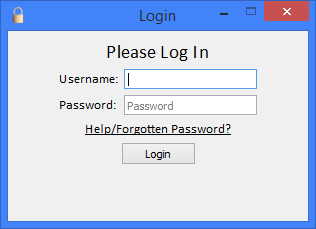
\includegraphics[width=\textwidth]{./Maintenance/UserInterface/LoginScreen.png}
\end{figure}

\begin{figure}[H]
    \caption{Forgot Password Screen} \label{fig:ForgotPasswordScreen}
    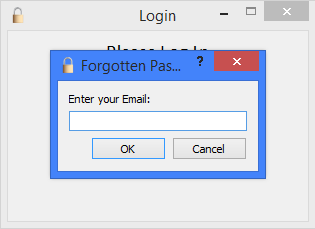
\includegraphics[width=\textwidth]{./Maintenance/UserInterface/ForgotPasswordScreen.png}
\end{figure}

\begin{figure}[H]
    \caption{Main Menu} \label{fig:MainMenu}
    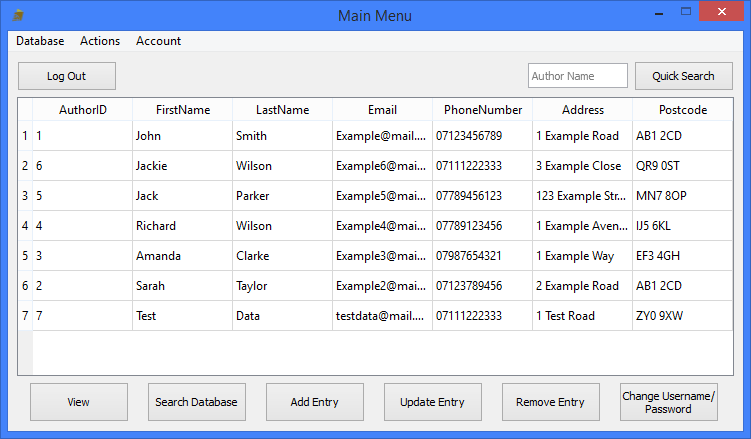
\includegraphics[width=\textwidth]{./Maintenance/UserInterface/MainMenu.png}
\end{figure}

\begin{figure}[H]
    \caption{Add Customer Entry} \label{fig:AddEntry}
    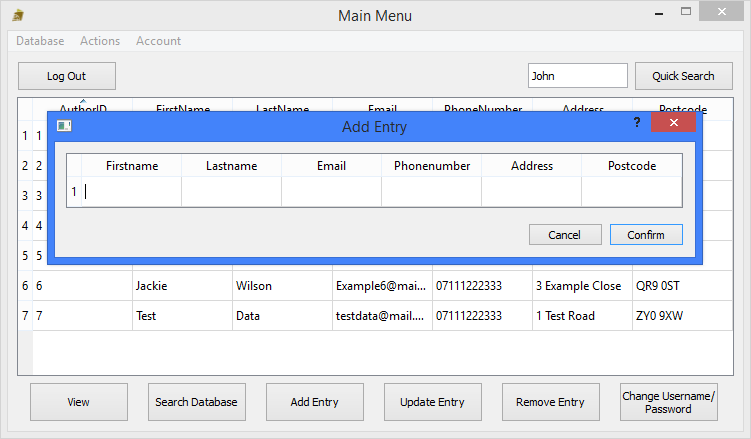
\includegraphics[width=\textwidth]{./Maintenance/UserInterface/AddEntry.png}
\end{figure}

\begin{figure}[H]
    \caption{Update Customer Entry} \label{fig:UpdateEntry}
    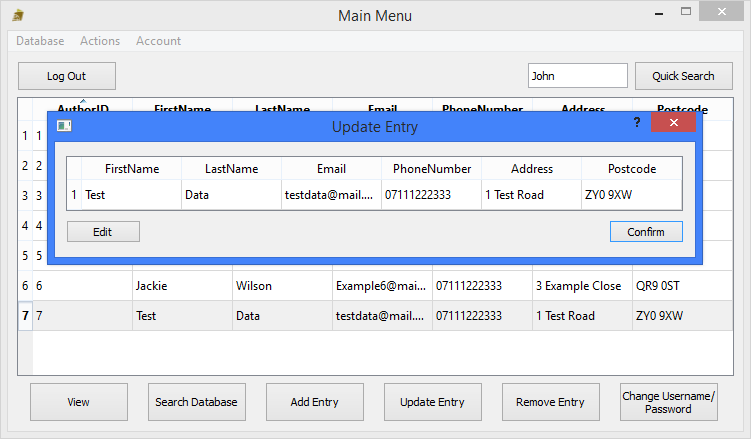
\includegraphics[width=\textwidth]{./Maintenance/UserInterface/UpdateEntry.png}
\end{figure}

\begin{figure}[H]
    \caption{Editing Customer Field} \label{fig:EditingEntry}
    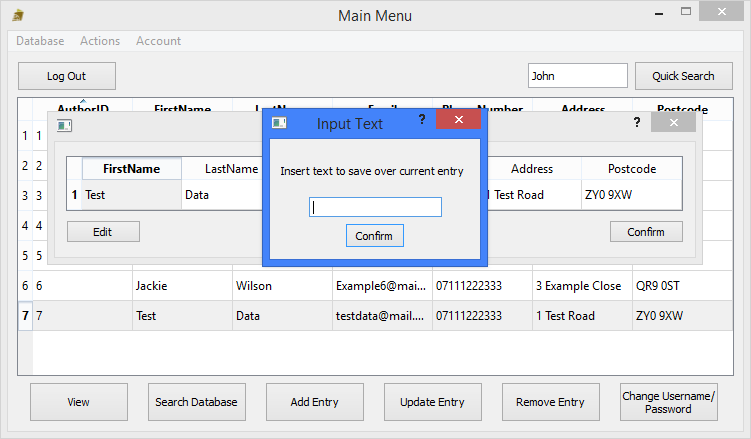
\includegraphics[width=\textwidth]{./Maintenance/UserInterface/EditingEntry.png}
\end{figure}

\begin{figure}[H]
    \caption{Update Customer Entry Verification} \label{fig:UpdateEntryVerify}
    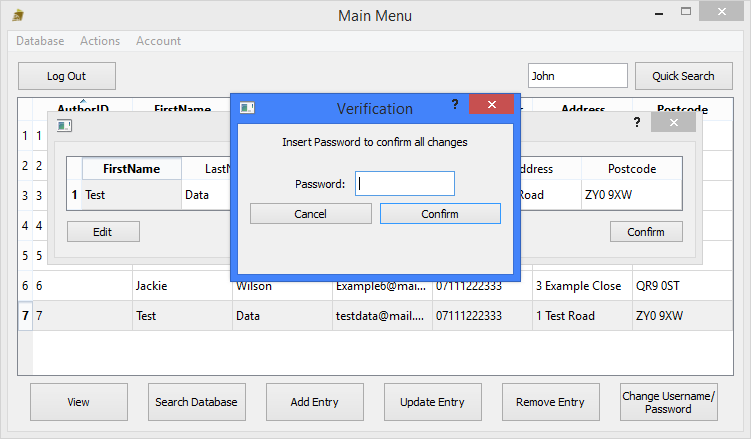
\includegraphics[width=\textwidth]{./Maintenance/UserInterface/UpdateEntryVerify.png}
\end{figure}

\begin{figure}[H]
    \caption{Update Customer Entry Success} \label{fig:UpdateEntrySuccess}
    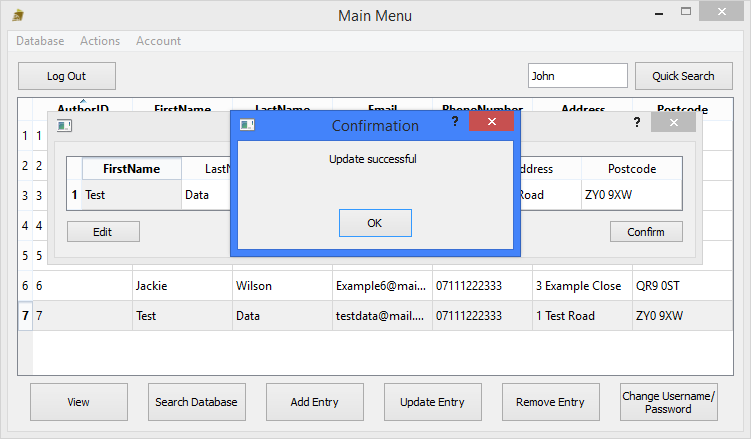
\includegraphics[width=\textwidth]{./Maintenance/UserInterface/UpdateEntrySuccess.png}
\end{figure}

\begin{figure}[H]
    \caption{Delete Customer Entry} \label{fig:DeleteEntry}
    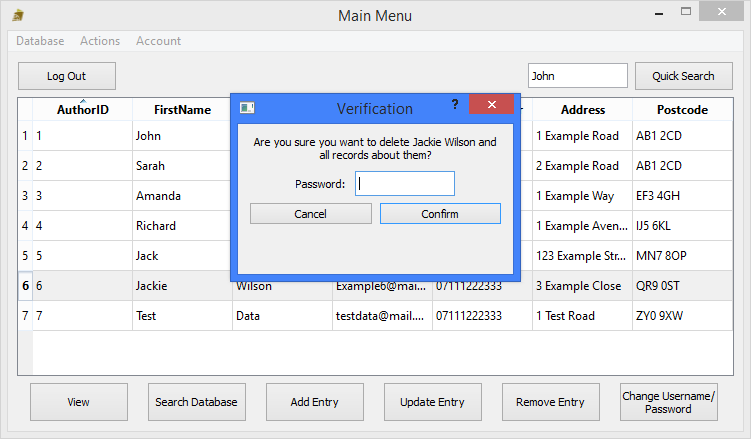
\includegraphics[width=\textwidth]{./Maintenance/UserInterface/DeleteEntry.png}
\end{figure}

\begin{figure}[H]
    \caption{Delete Entry Success} \label{fig:DeleteEntrySuccess}
    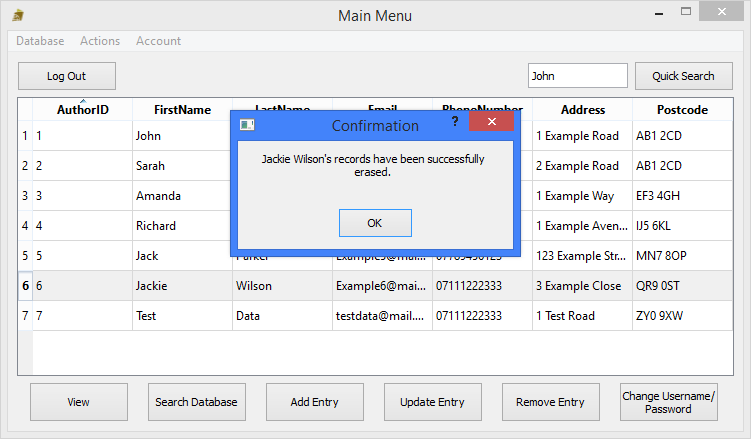
\includegraphics[width=\textwidth]{./Maintenance/UserInterface/DeleteEntrySuccess.png}
\end{figure}

\begin{figure}[H]
    \caption{View Menu} \label{fig:ViewMenu}
    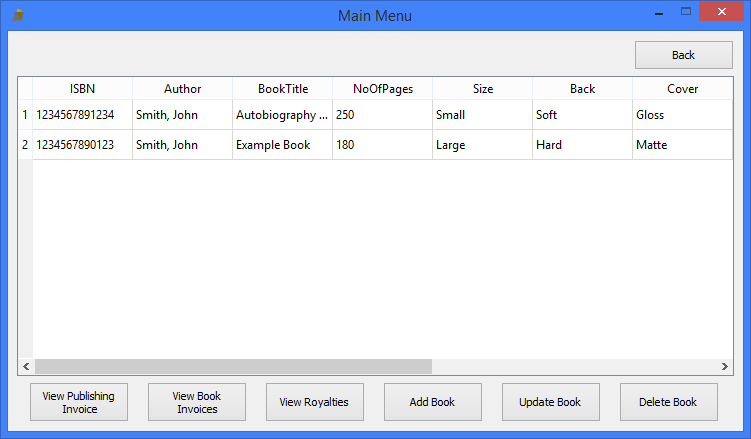
\includegraphics[width=\textwidth]{./Maintenance/UserInterface/ViewMenu.png}
\end{figure}

\begin{figure}[H]
    \caption{View Publishing Invoices} \label{fig:ViewPubInvoices}
    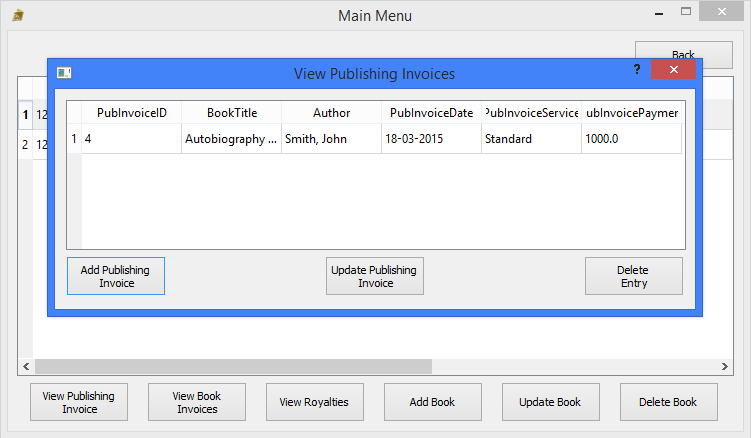
\includegraphics[width=\textwidth]{./Maintenance/UserInterface/ViewPubInvoices.png}
\end{figure}

\begin{figure}[H]
    \caption{Add Publishing Invoice} \label{fig:AddPubInvoice}
    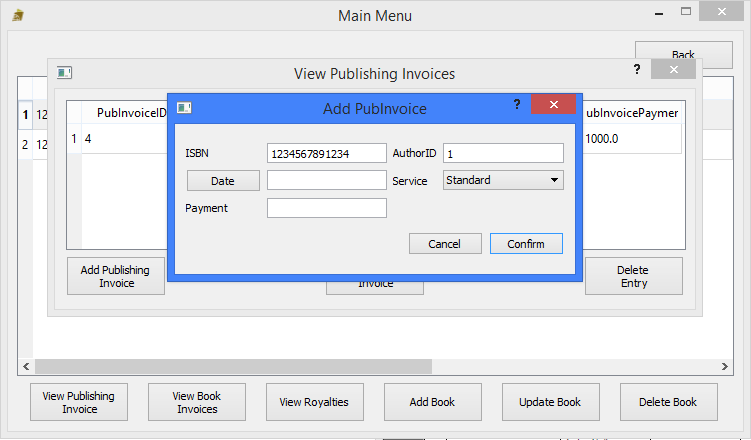
\includegraphics[width=\textwidth]{./Maintenance/UserInterface/AddPubInvoice.png}
\end{figure}

\begin{figure}[H]
    \caption{Update Publishing Invoice} \label{fig:UpdatePubInvoice}
    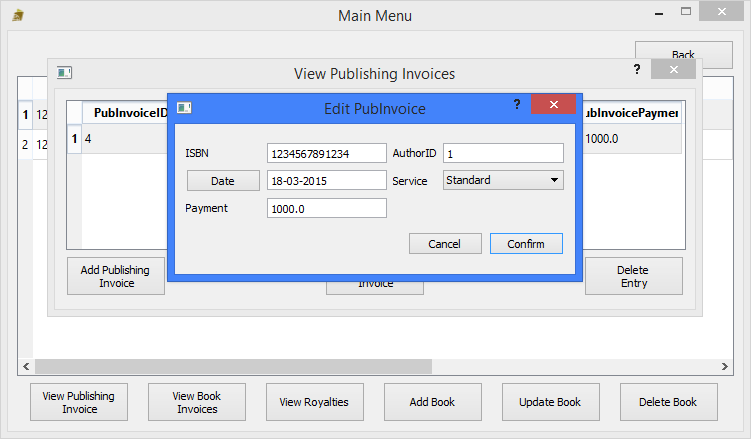
\includegraphics[width=\textwidth]{./Maintenance/UserInterface/UpdatePubInvoice.png}
\end{figure}

\begin{figure}[H]
    \caption{Update Verification} \label{fig:UpdatePubInvoiceVerify}
    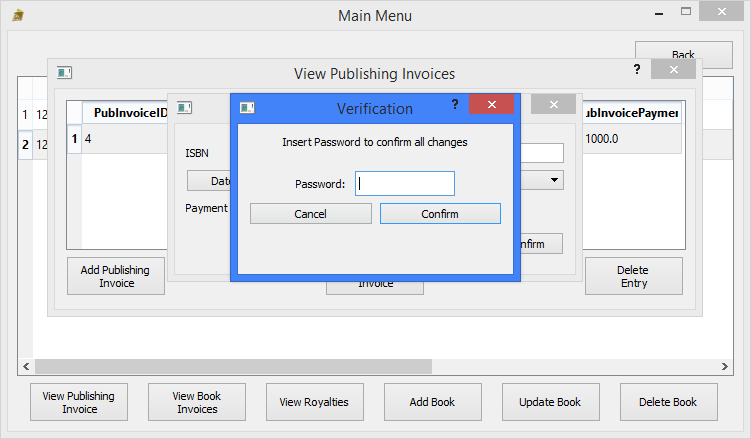
\includegraphics[width=\textwidth]{./Maintenance/UserInterface/UpdatePubInvoiceVerify.png}
\end{figure}

\begin{figure}[H]
    \caption{Update Success} \label{fig:UpdatePubInvoiceSuccess}
    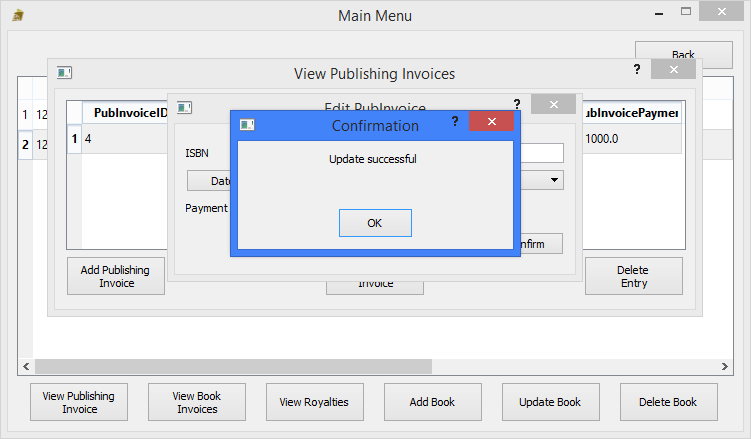
\includegraphics[width=\textwidth]{./Maintenance/UserInterface/UpdatePubInvoiceSuccess.png}
\end{figure}

\begin{figure}[H]
    \caption{Delete Verification} \label{fig:DeletePubInvoice}
    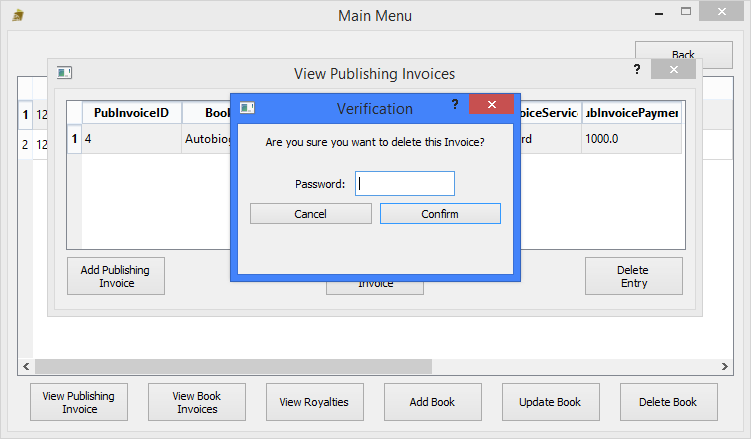
\includegraphics[width=\textwidth]{./Maintenance/UserInterface/DeletePubInvoice.png}
\end{figure}

\begin{figure}[H]
    \caption{Delete Success} \label{fig:DeletePubInvoiceSuccess}
    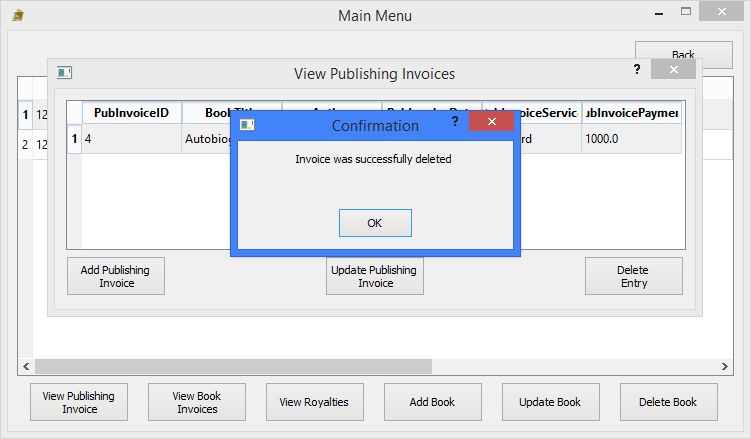
\includegraphics[width=\textwidth]{./Maintenance/UserInterface/DeletePubInvoiceSuccess.png}
\end{figure}

\begin{figure}[H]
    \caption{View Book Invoices} \label{fig:ViewBookInvoices}
    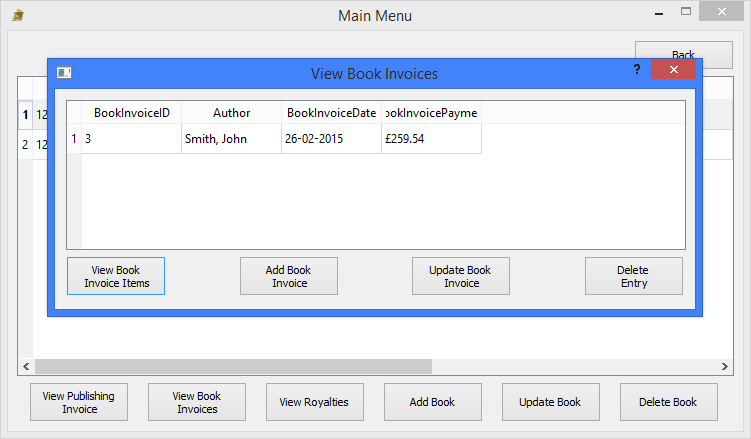
\includegraphics[width=\textwidth]{./Maintenance/UserInterface/ViewBookInvoices.png}
\end{figure}

\begin{figure}[H]
    \caption{Add Book Invoice} \label{fig:AddBookInvoice}
    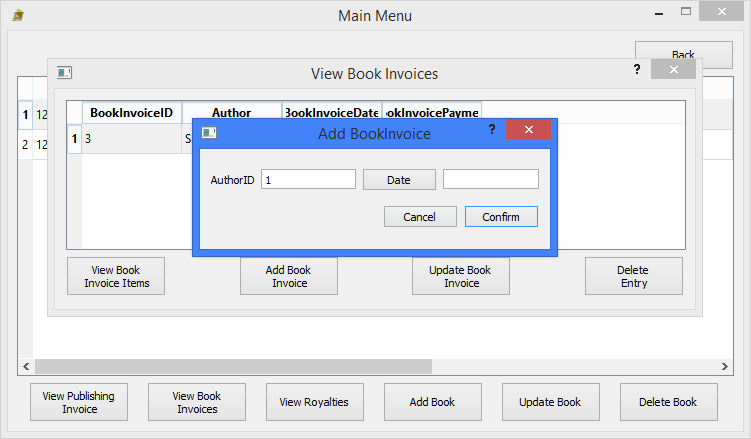
\includegraphics[width=\textwidth]{./Maintenance/UserInterface/AddBookInvoice.png}
\end{figure}

\begin{figure}[H]
    \caption{Update Book Invoice} \label{fig:UpdateBookInvoice}
    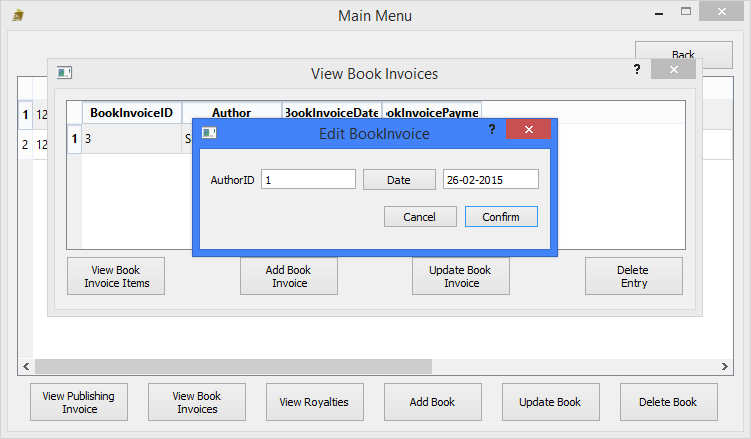
\includegraphics[width=\textwidth]{./Maintenance/UserInterface/UpdateBookInvoice.png}
\end{figure}

\begin{figure}[H]
    \caption{View Book Invoice Items} \label{fig:ViewBookInvoiceItems}
    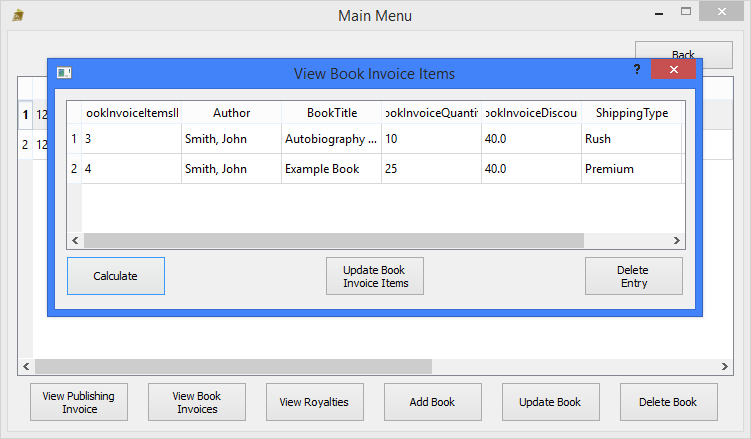
\includegraphics[width=\textwidth]{./Maintenance/UserInterface/ViewBookInvoiceItems.png}
\end{figure}

\begin{figure}[H]
    \caption{Add Book Invoice Items} \label{fig:AddBookInvoiceItems}
    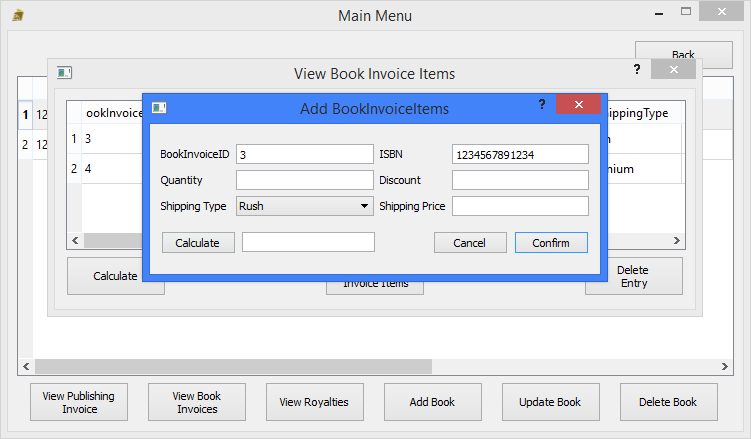
\includegraphics[width=\textwidth]{./Maintenance/UserInterface/AddBookInvoiceItems.png}
\end{figure}

\begin{figure}[H]
    \caption{Update Book Invoice Items} \label{fig:UpdateBookInvoiceItems}
    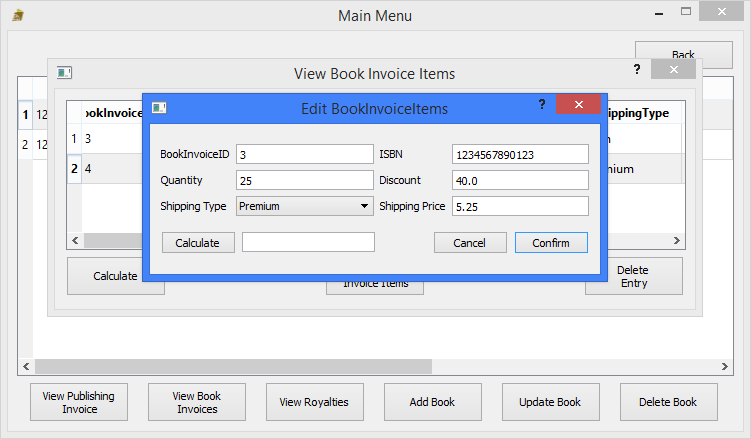
\includegraphics[width=\textwidth]{./Maintenance/UserInterface/UpdateBookInvoiceItems.png}
\end{figure}

\begin{figure}[H]
    \caption{View Royalties} \label{fig:ViewRoyalties}
    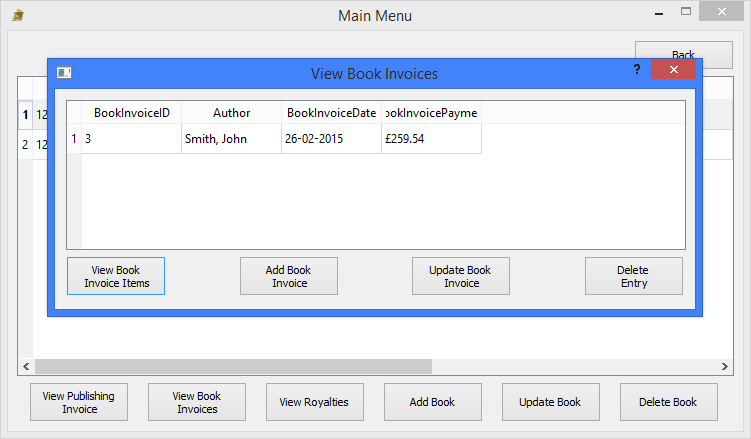
\includegraphics[width=\textwidth]{./Maintenance/UserInterface/ViewBookInvoices.png}
\end{figure}

\begin{figure}[H]
    \caption{Add Royalties} \label{fig:AddRoyalties}
    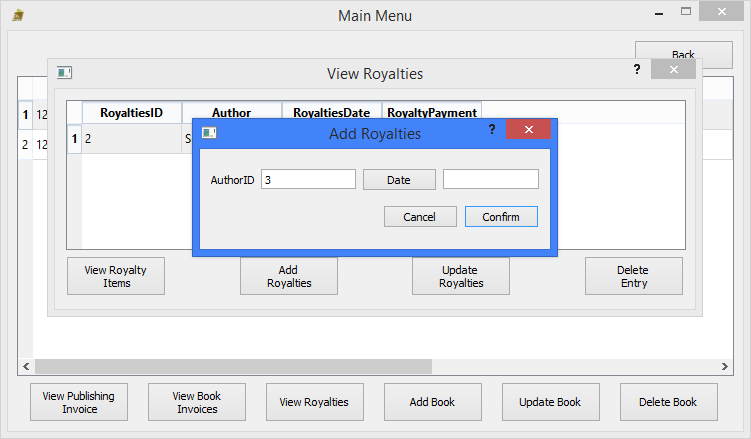
\includegraphics[width=\textwidth]{./Maintenance/UserInterface/AddRoyalties.png}
\end{figure}

\begin{figure}[H]
    \caption{Update Royalties} \label{fig:UpdateRoyalties}
    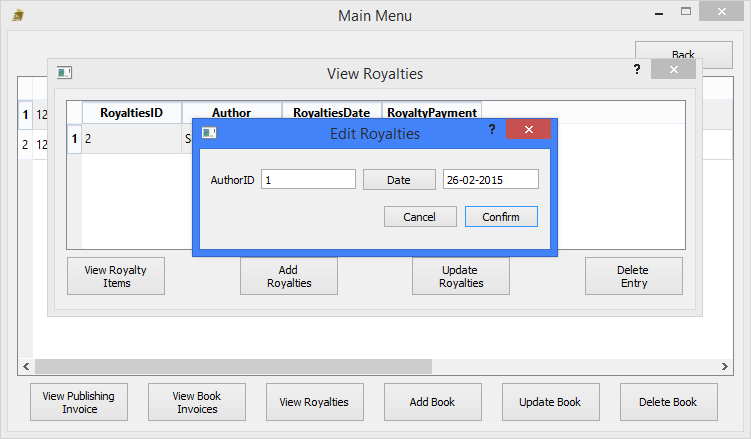
\includegraphics[width=\textwidth]{./Maintenance/UserInterface/UpdateRoyalties.png}
\end{figure}

\begin{figure}[H]
    \caption{View Royalty Items} \label{fig:ViewRoyaltyItems}
    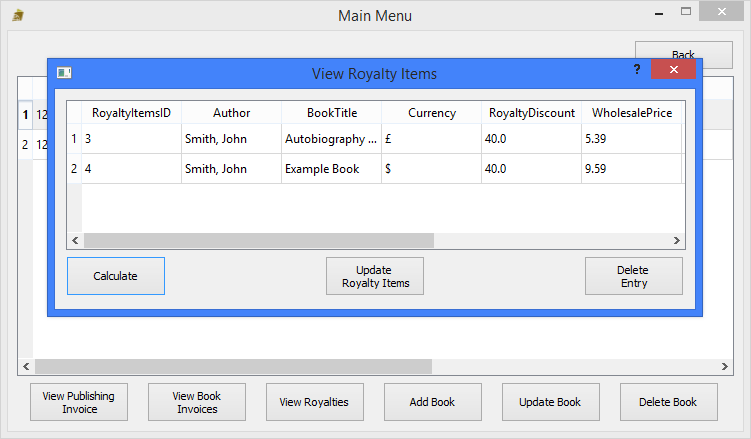
\includegraphics[width=\textwidth]{./Maintenance/UserInterface/ViewRoyaltyItems.png}
\end{figure}

\begin{figure}[H]
    \caption{Add Royalty Items} \label{fig:AddRoyaltyItems}
    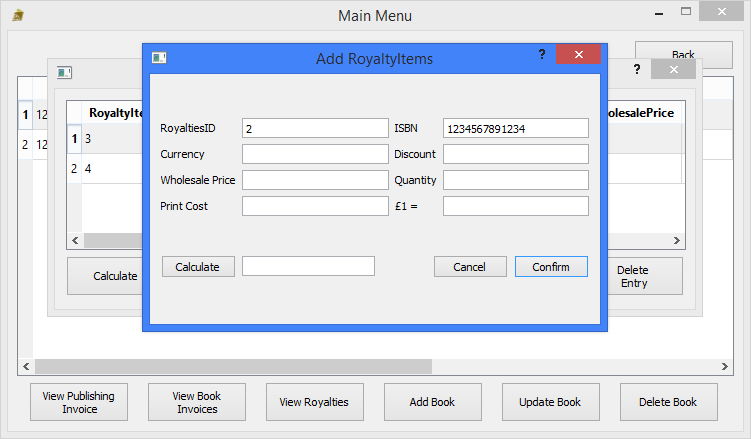
\includegraphics[width=\textwidth]{./Maintenance/UserInterface/AddRoyaltyItems.png}
\end{figure}

\begin{figure}[H]
    \caption{Update Royalty Items} \label{fig:UpdateRoyaltyItems}
    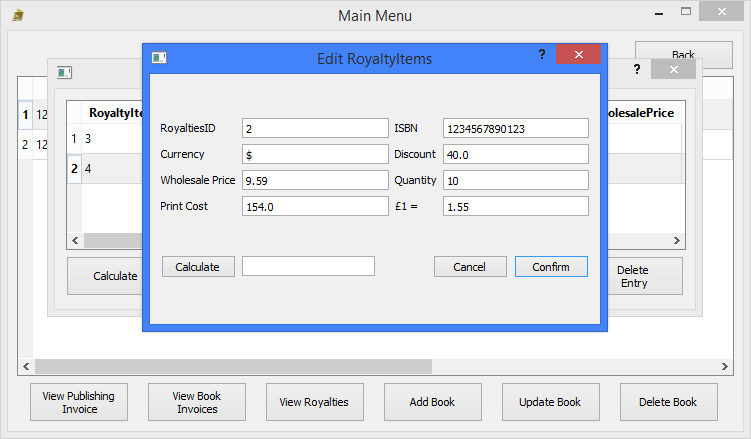
\includegraphics[width=\textwidth]{./Maintenance/UserInterface/UpdateRoyaltyItems.png}
\end{figure}

\begin{figure}[H]
    \caption{Add Book} \label{fig:AddBook}
    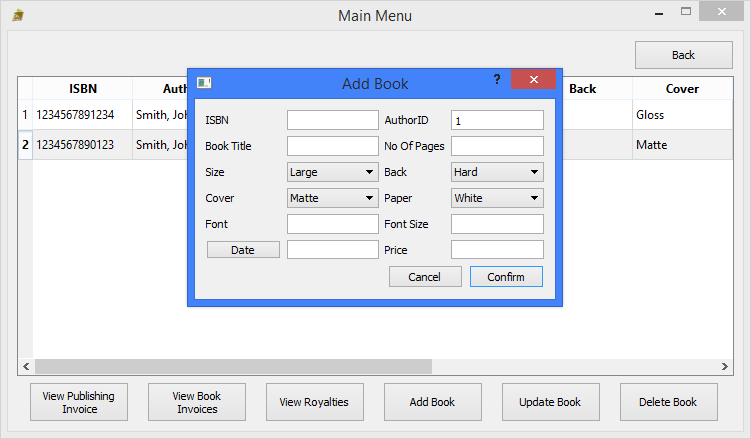
\includegraphics[width=\textwidth]{./Maintenance/UserInterface/AddBook.png}
\end{figure}

\begin{figure}[H]
    \caption{Update Book} \label{fig:UpdateBook}
    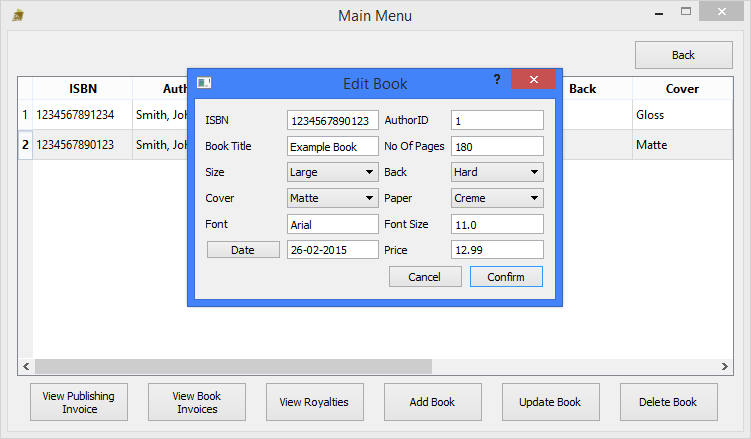
\includegraphics[width=\textwidth]{./Maintenance/UserInterface/UpdateBook.png}
\end{figure}

\begin{figure}[H]
    \caption{Quick Search} \label{fig:QuickSearch}
    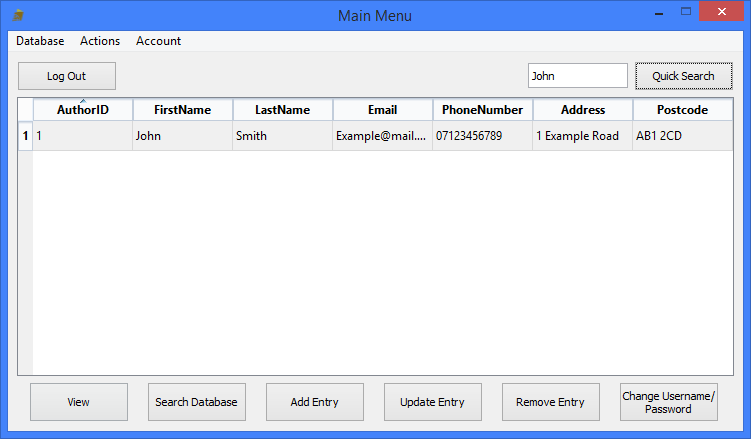
\includegraphics[width=\textwidth]{./Maintenance/UserInterface/QuickSearch.png}
\end{figure}

\begin{figure}[H]
    \caption{Selection For Changing User Credentials} \label{fig:ChangeSelection}
    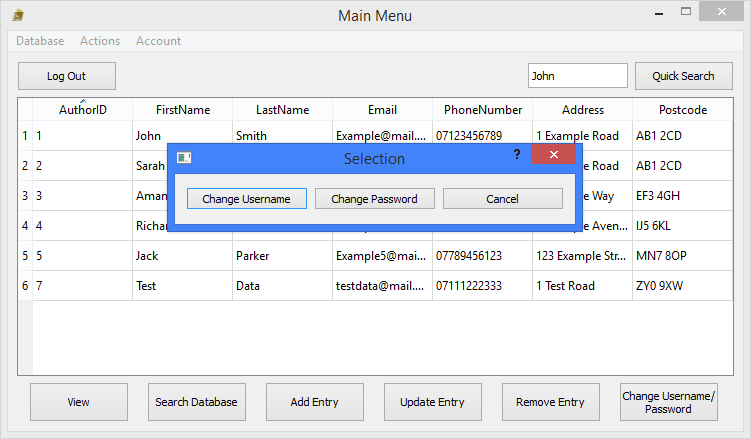
\includegraphics[width=\textwidth]{./Maintenance/UserInterface/ChangeSelection.png}
\end{figure}

\begin{figure}[H]
    \caption{Change Username} \label{fig:ChangeUsername}
    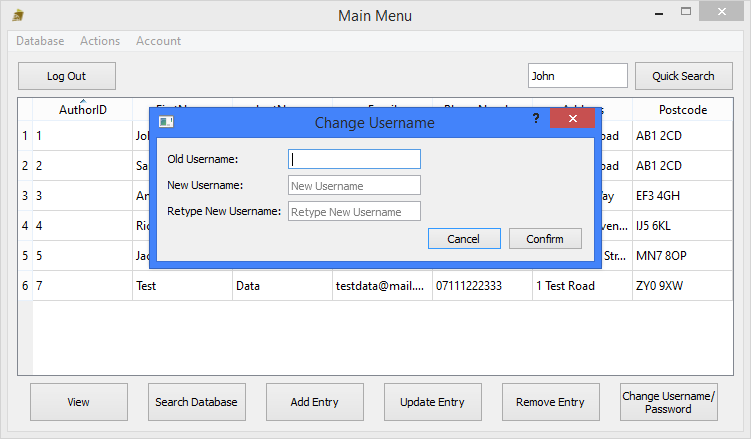
\includegraphics[width=\textwidth]{./Maintenance/UserInterface/ChangeUsername.png}
\end{figure}

\begin{figure}[H]
    \caption{Change Username Success} \label{fig:ChangeUsernameSuccess}
    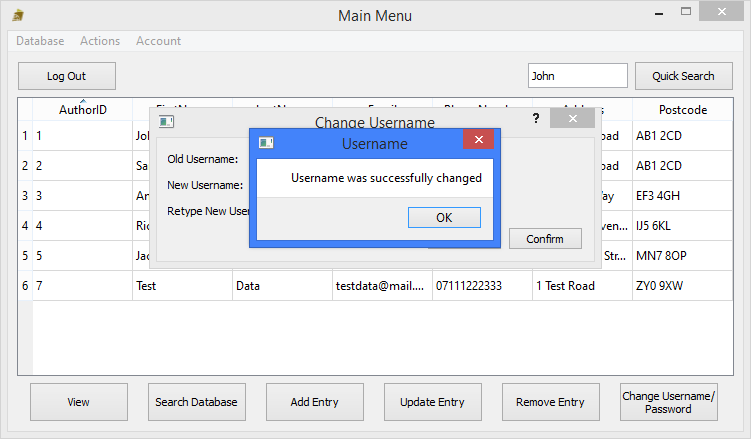
\includegraphics[width=\textwidth]{./Maintenance/UserInterface/ChangeUsernameSuccess.png}
\end{figure}

\begin{figure}[H]
    \caption{Change Password} \label{fig:ChangePassword}
    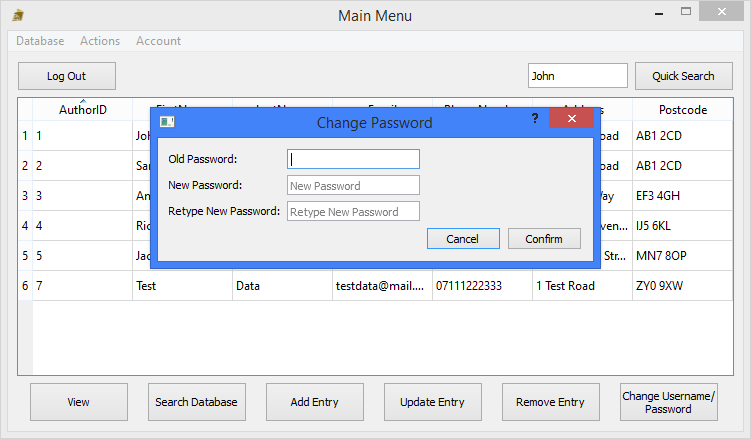
\includegraphics[width=\textwidth]{./Maintenance/UserInterface/ChangePassword.png}
\end{figure}

\begin{figure}[H]
    \caption{Change Password Success} \label{fig:ChangePasswordSuccess}
    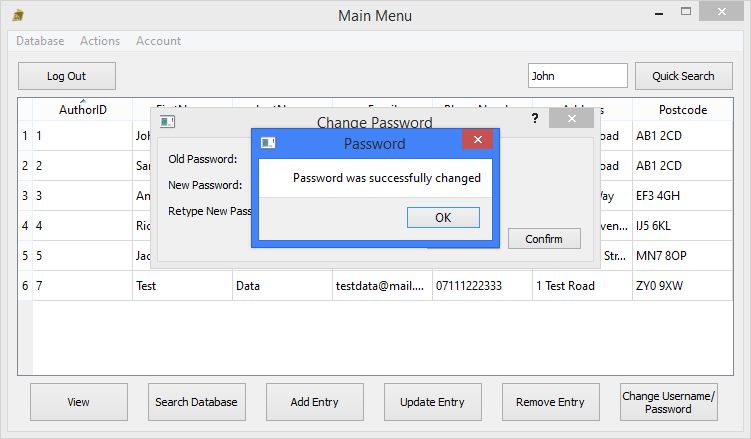
\includegraphics[width=\textwidth]{./Maintenance/UserInterface/ChangePasswordSuccess.png}
\end{figure}

\begin{figure}[H]
    \caption{Search} \label{fig:Search}
    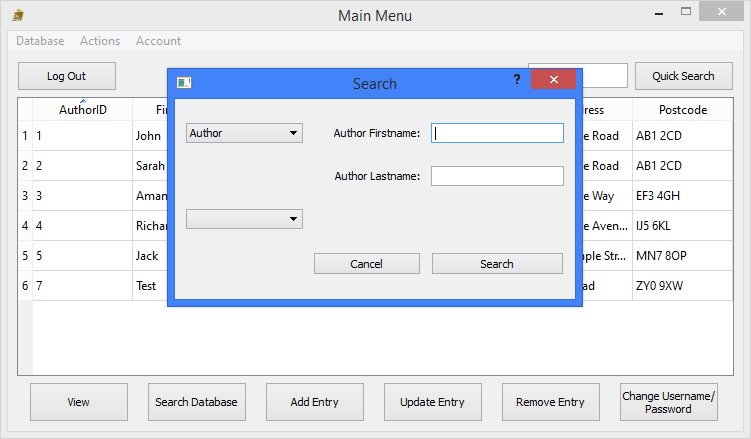
\includegraphics[width=\textwidth]{./Maintenance/UserInterface/Search.png}
\end{figure}

\begin{figure}[H]
    \caption{Search with a different selection to Author} \label{fig:SearchSelectionChosen}
    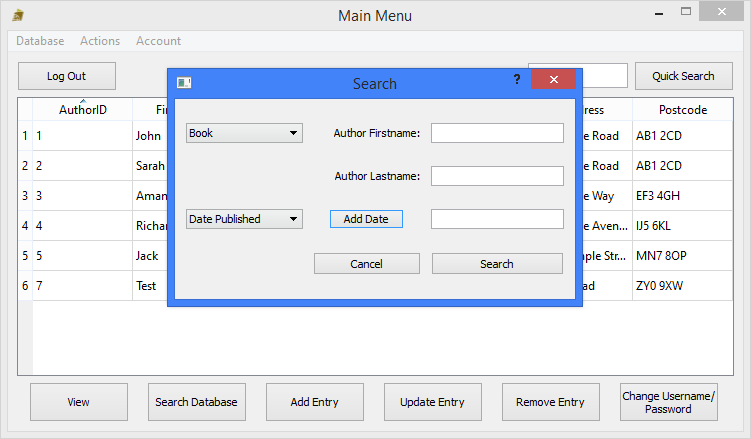
\includegraphics[width=\textwidth]{./Maintenance/UserInterface/SearchSelectionChosen.png}
\end{figure}

\begin{figure}[H]
    \caption{No Match Found For Search} \label{fig:NoMatchSearch}
    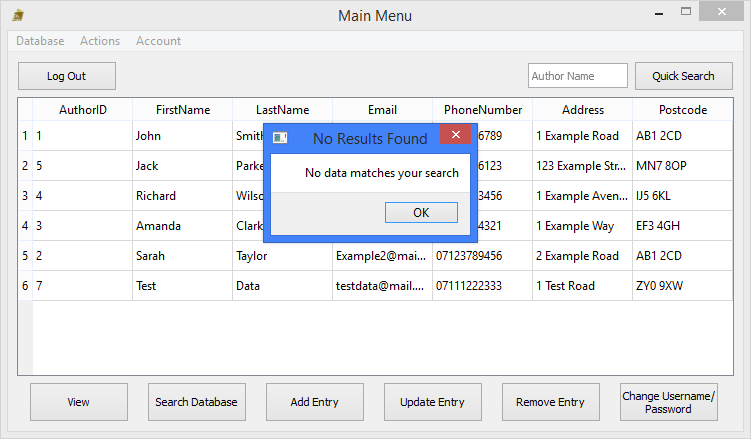
\includegraphics[width=\textwidth]{./Maintenance/UserInterface/NoMatchSearch.png}
\end{figure}

\begin{figure}[H]
    \caption{Search Results Example} \label{fig:SearchExample}
    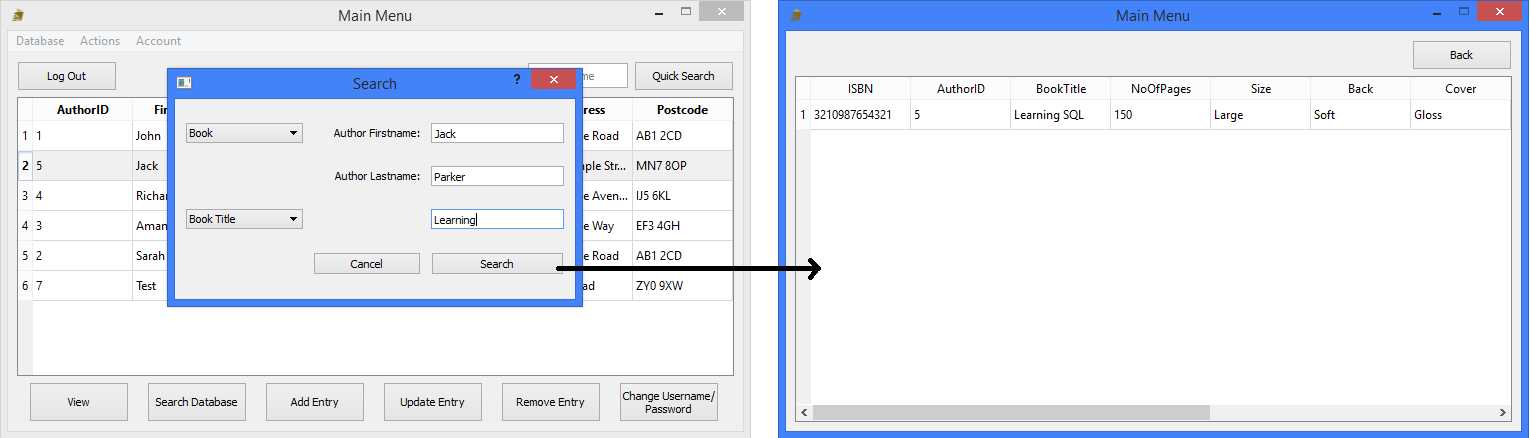
\includegraphics[width=\textwidth]{./Maintenance/UserInterface/SearchExample.png}
\end{figure}

\subsection{ER Diagram}

\begin{figure}[H]
    \caption{ER Diagram} \label{ER_Diagram.pdf}
    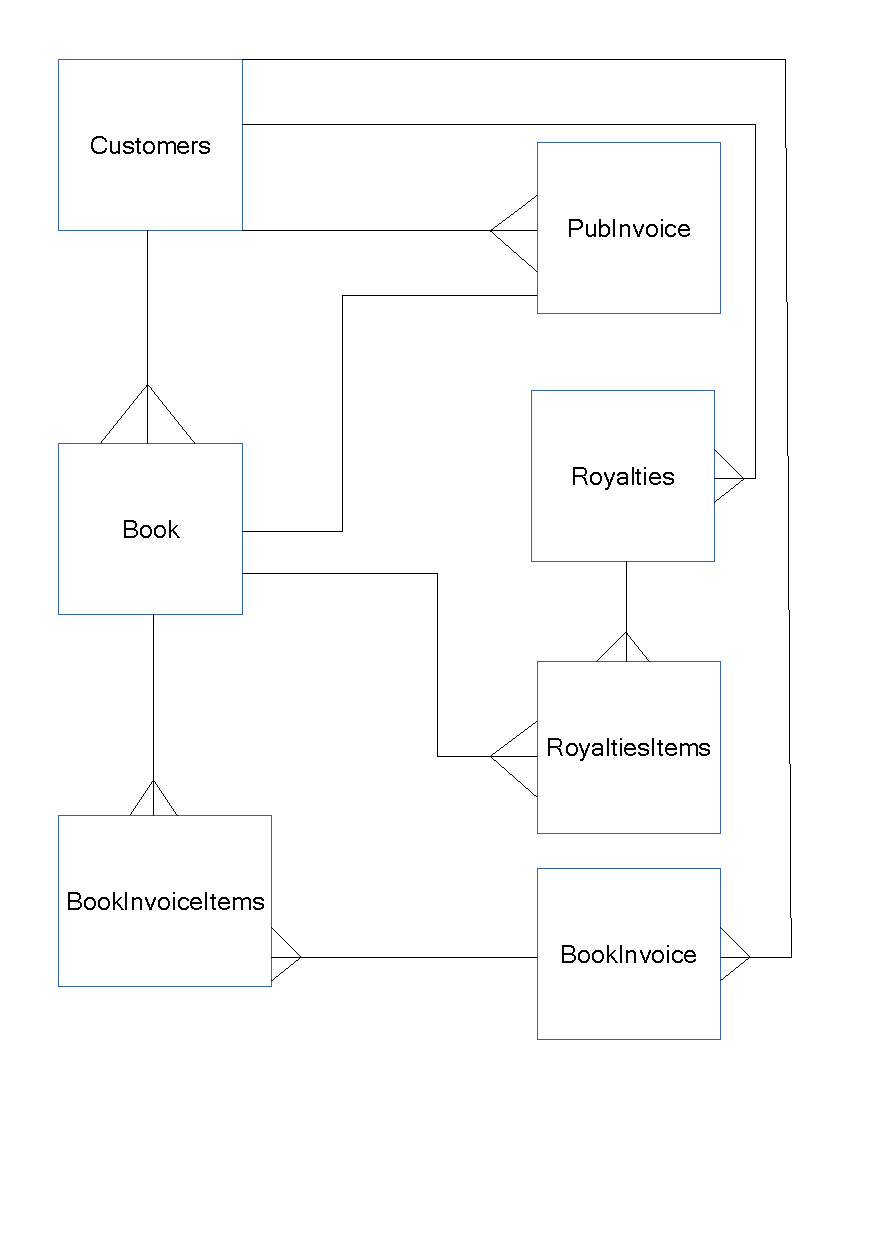
\includegraphics[width=\textwidth]{./Design/ER_Diagram.pdf}
\end{figure}

\subsection{Database Table Views}

\begin{figure}[H]
    \caption{Customer} \label{fig:Customer}
    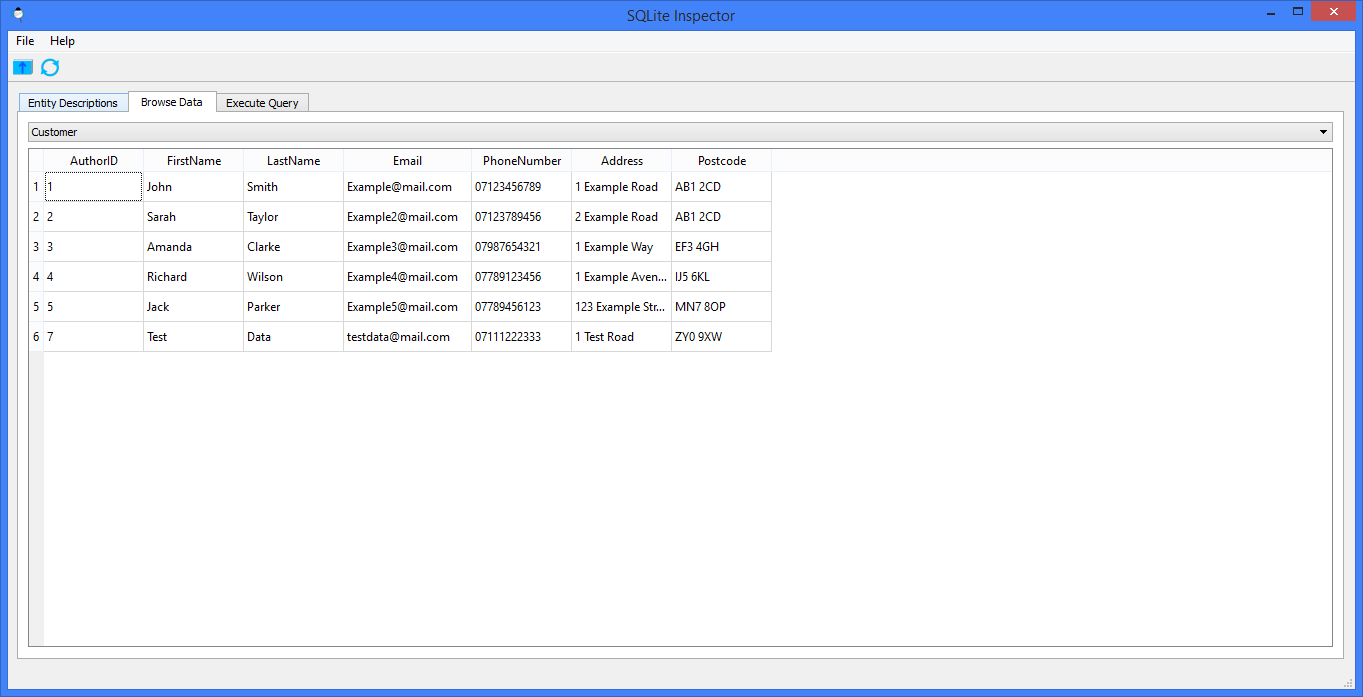
\includegraphics[width=\textwidth]{./Maintenance/DatabaseTables/Customer.png}
\end{figure}

\begin{figure}[H]
    \caption{Book} \label{fig:Book}
    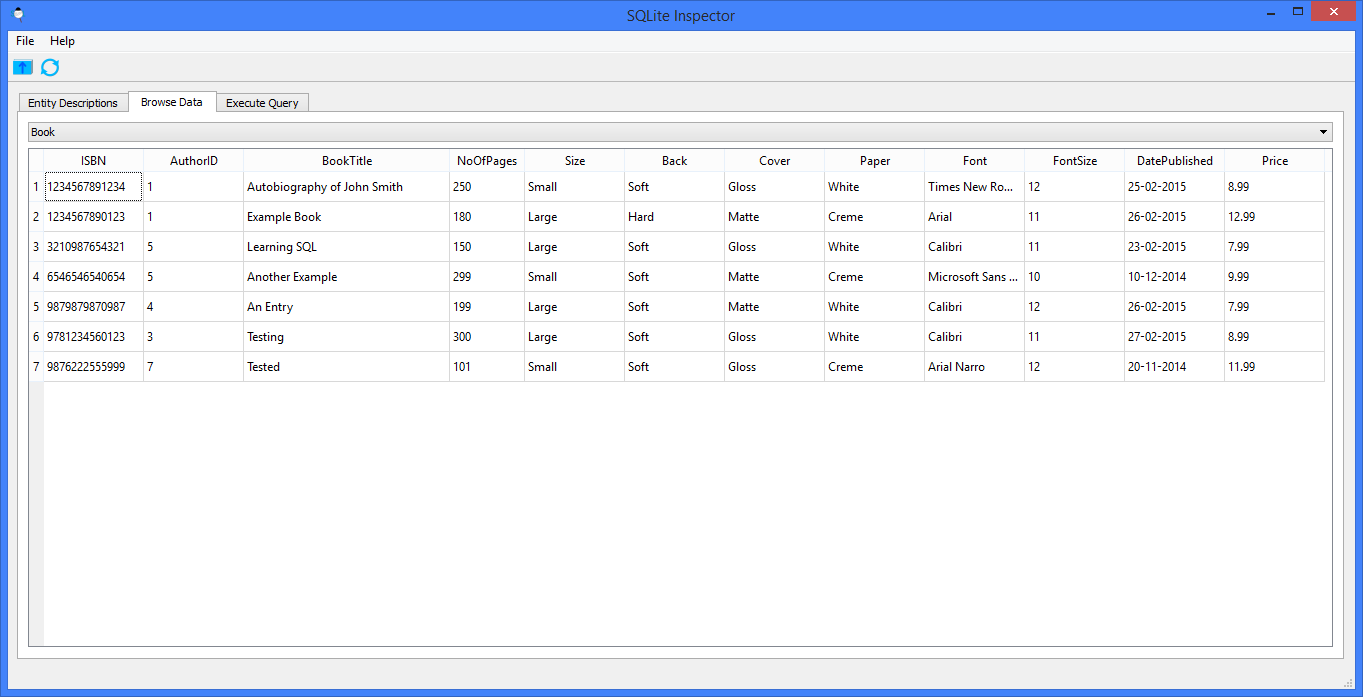
\includegraphics[width=\textwidth]{./Maintenance/DatabaseTables/Book.png}
\end{figure}

\begin{figure}[H]
    \caption{Publishing Invoice} \label{fig:PubInvoice}
    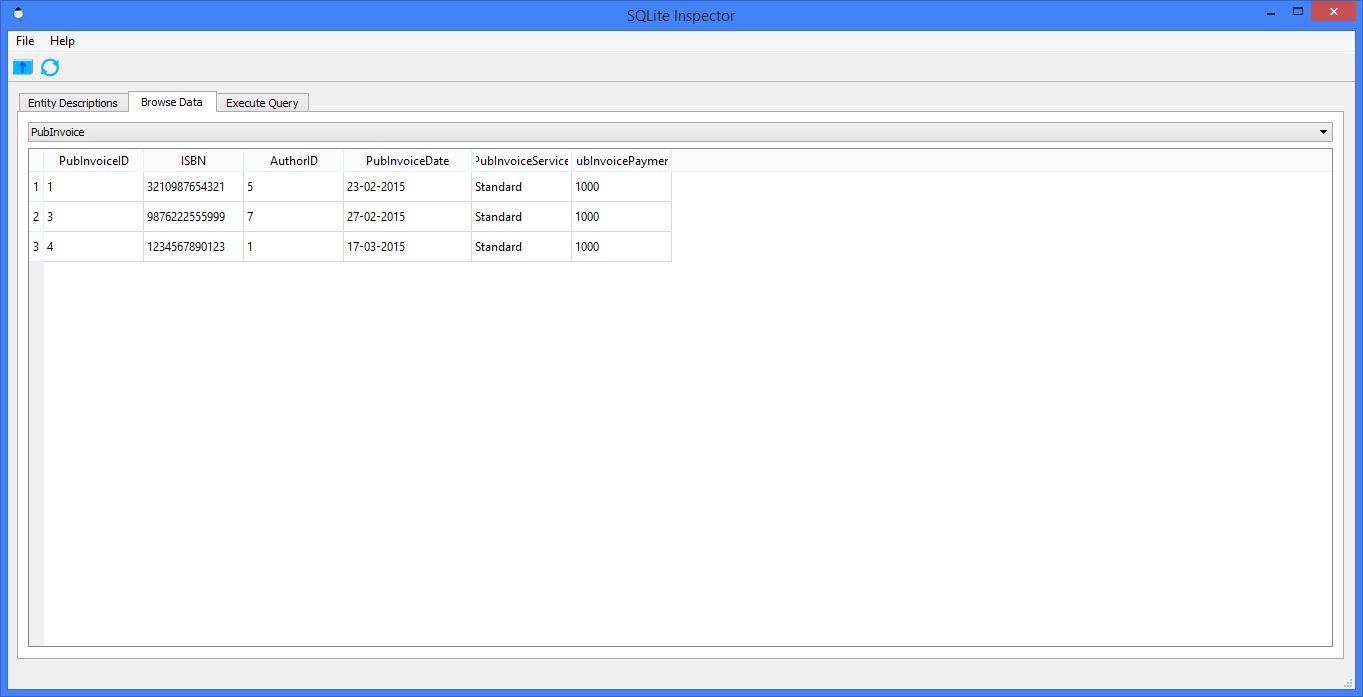
\includegraphics[width=\textwidth]{./Maintenance/DatabaseTables/PubInvoice.png}
\end{figure}

\begin{figure}[H]
    \caption{Book Invoice} \label{fig:BookInvoice}
    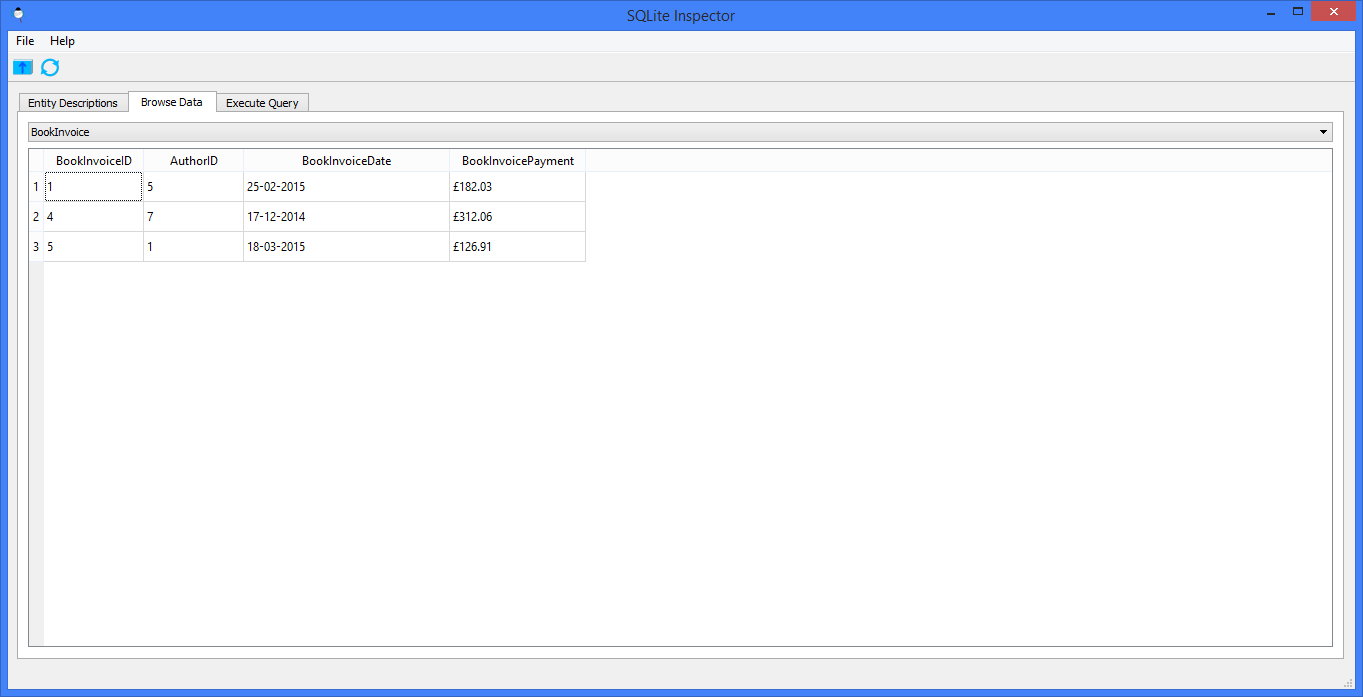
\includegraphics[width=\textwidth]{./Maintenance/DatabaseTables/BookInvoice.png}
\end{figure}

\begin{figure}[H]
    \caption{Book Invoice Items} \label{fig:BookInvoiceItems}
    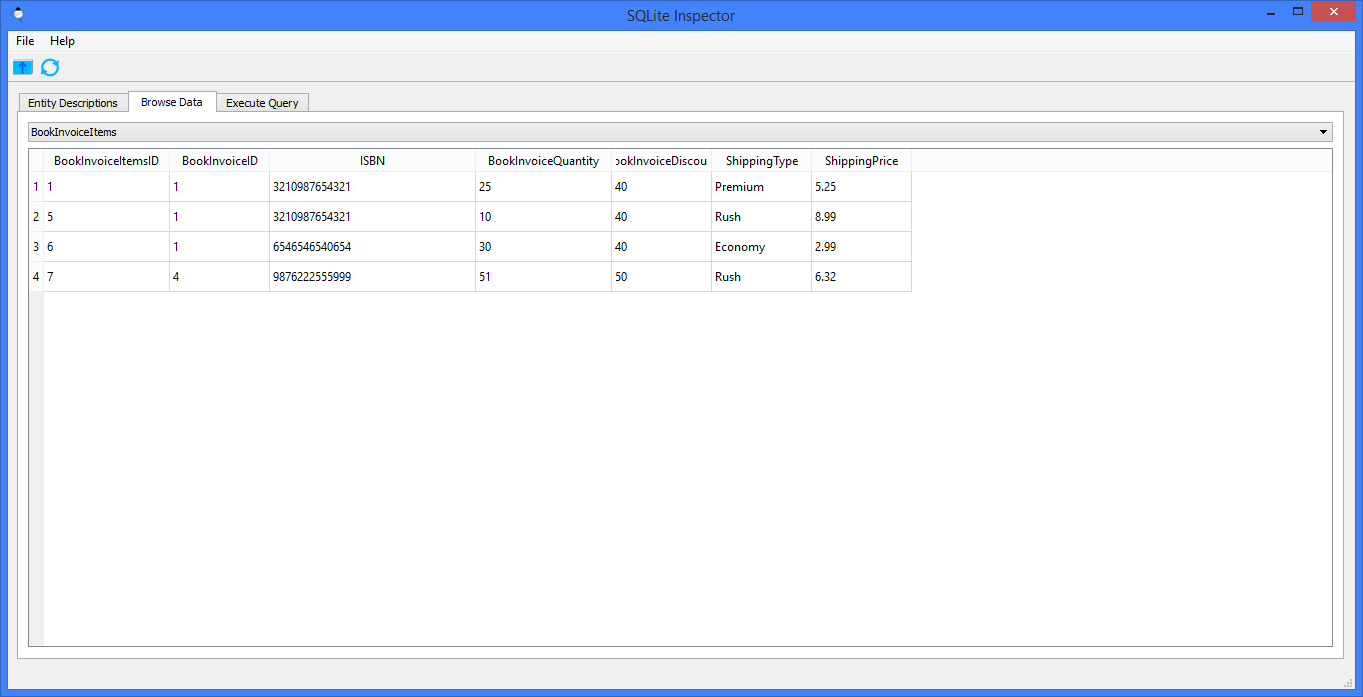
\includegraphics[width=\textwidth]{./Maintenance/DatabaseTables/BookInvoiceItems.png}
\end{figure}

\begin{figure}[H]
    \caption{Royalties} \label{fig:Royalties}
    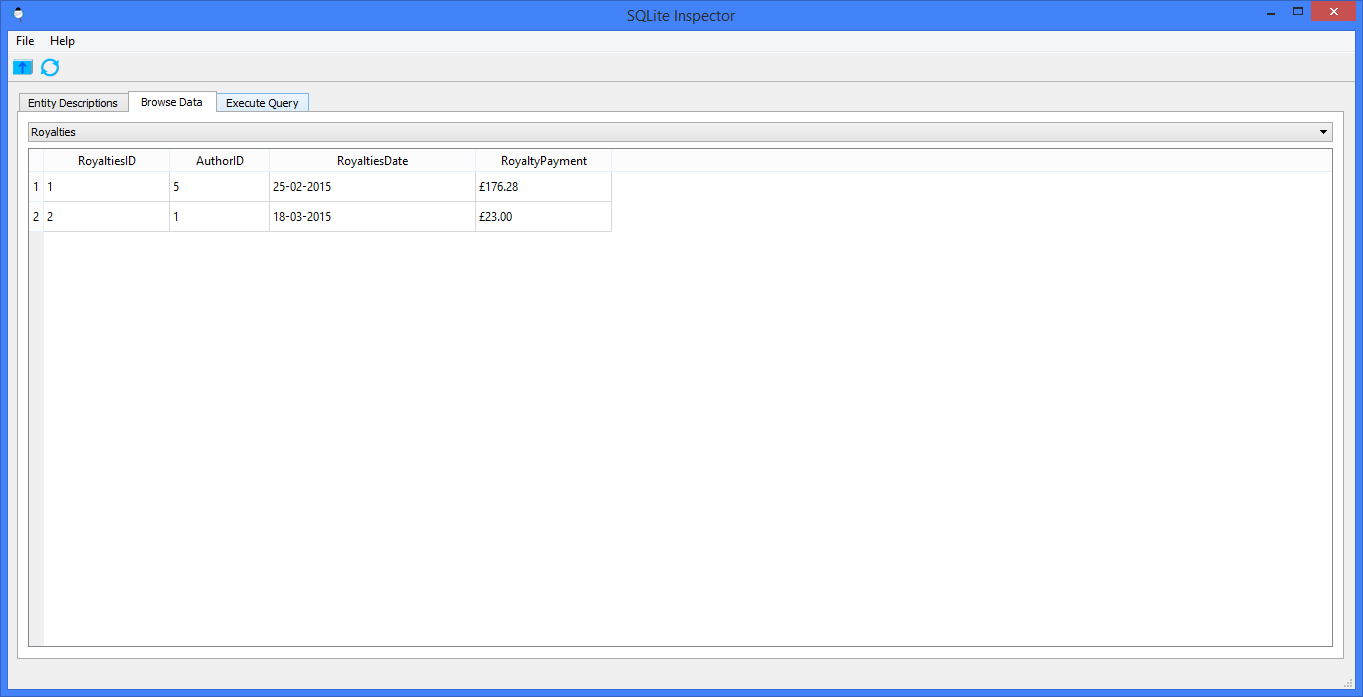
\includegraphics[width=\textwidth]{./Maintenance/DatabaseTables/Royalties.png}
\end{figure}

\begin{figure}[H]
    \caption{Royalty Items} \label{fig:Royalty Items}
    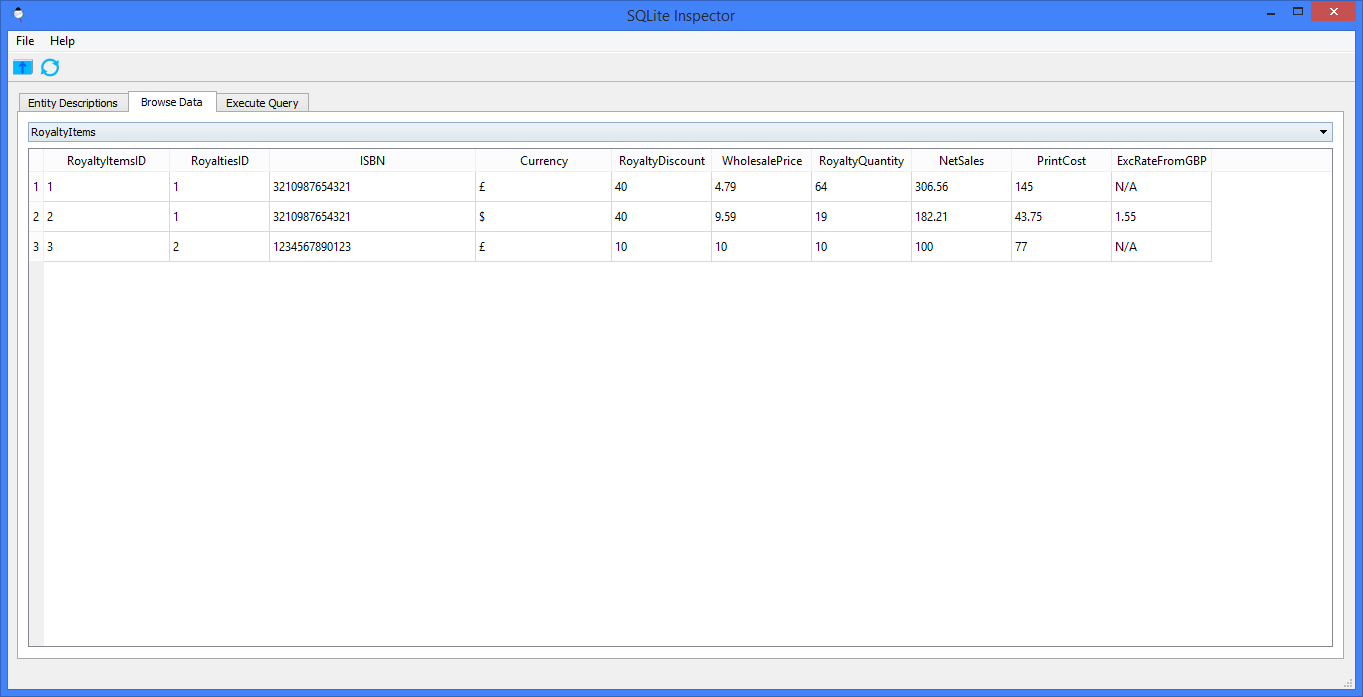
\includegraphics[width=\textwidth]{./Maintenance/DatabaseTables/RoyaltyItems.png}
\end{figure}

\subsection{Database SQL}

The following SQL statements can be found in Module 1,  subsection \ref{ssec:LoginDB.py}

Creating Customer Table:
\begin{sql}
CREATE TABLE Customer 
                 (AuthorID integer,
                 FirstName text,
                 LastName text,
                 Email text,
                 PhoneNumber text,
                 Address text,
                 Postcode text,
                 primary key(AuthorID))
\end{sql}

Creating Book Table:
\begin{sql}
CREATE TABLE Book 
                 (ISBN text,
                 AuthorID integer,
                 BookTitle text,
                 NoOfPages integer,
                 Size text,
                 Back text,
                 Cover text,
                 Paper text,
                 Font text,
                 FontSize real,
                 DatePublished date,
                 Price real,
                 primary key(ISBN),
                 foreign key(AuthorID) references Customer(AuthorID))
\end{sql}

Creating Publishing Invoice Table:
\begin{sql}
CREATE TABLE PubInvoice 
                 (PubInvoiceID integer,
                 ISBN text,
                 AuthorID integer,
                 PubInvoiceDate date,
                 PubInvoiceService text,
                 PubInvoicePayment real,
                 primary key(PubInvoiceID),
                 foreign key(AuthorID) references Customer(AuthorID),
                 foreign key(ISBN) references Book(ISBN))
\end{sql}

Creating Book Invoice Table:
\begin{sql}
CREATE TABLE BookInvoice
                 (BookInvoiceID integer,
                 AuthorID integer,
                 BookInvoiceDate date,
                 BookInvoicePayment real,
                 primary key(BookInvoiceID),
                 foreign key(AuthorID) references Customer(AuthorID))
\end{sql}

Creating Book Invoice Items Table:
\begin{sql}
CREATE TABLE BookInvoiceItems
                 (BookInvoiceItemsID integer,
                 BookInvoiceID integer,
                 ISBN text,
                 BookInvoiceQuantity integer,
                 BookInvoiceDiscount real,
                 ShippingType text,
                 ShippingPrice real,
                 primary key(BookInvoiceItemsID),
                 foreign key(BookInvoiceID) references BookInvoice(BookInvoiceID),
                 foreign key(ISBN) references Book(ISBN))
\end{sql}

Creating Royalties Table:
\begin{sql}
CREATE TABLE Royalties
                 (RoyaltiesID integer,
                 AuthorID integer,
                 RoyaltiesDate date,
                 RoyaltyPayment real,
                 primary key(RoyaltiesID),
                 foreign key(AuthorID) references Customer(AuthorID))
\end{sql}

Creating Royalty Items Table:
\begin{sql}
CREATE TABLE RoyaltyItems
                 (RoyaltyItemsID integer,
                 RoyaltiesID integer,
                 ISBN text,
                 Currency text,
                 RoyaltyDiscount real,
                 WholesalePrice real,
                 RoyaltyQuantity integer,
                 NetSales real,
                 PrintCost real,
                 ExcRateFromGBP real,
                 primary key(RoyaltyItemsID),
                 foreign key(RoyaltiesID) references Royalties(RoyaltiesID),
                 foreign key(ISBN) references Book(ISBN))
\end{sql}

Creating a Login Details Table if it does not exist, for login purposes:
\begin{sql}
CREATE TABLE if not exists LoginDetails
                 (Username text
                 Password text)
\end{sql}

\subsection{SQL Queries}

Checking whether the login table is existent:
\begin{sql}
select name
from sqlite_master
where type='table' and name='LoginDetails'
\end{sql}
Reference: Module 1,  subsection \ref{ssec:LoginDB.py}, line 35.

\

Creating the default Username and Password.
\begin{sql}
insert into LoginDetails (Username, Password)
values (?, ?)
\end{sql}
Reference: Module 1,  subsection \ref{ssec:LoginDB.py}, line 47.

\

Fetching the current username:
\begin{sql}
select Username
from LoginDetails
\end{sql}
Reference: Module 1,  subsection \ref{ssec:LoginDB.py}, line 108.

\

Fetching the current password:
\begin{sql}
select Password
from LoginDetails
\end{sql}
Reference: Module 1,  subsection \ref{ssec:LoginDB.py}, line 110.

\

Fetching all Customer data:
\begin{sql}
select *
from Customer
\end{sql}
Reference: Module 2,  subsection \ref{ssec:MainMenu.py}, line 38.

\

Fetching all Book data:
\begin{sql}
select *
from Book
\end{sql}
Reference: Module 2,  subsection \ref{ssec:MainMenu.py}, line 111.

\

Selecting data to be entered by user for PubInvoice:
\begin{sql}
select ISBN, AuthorID, PubInvoiceDate, PubInvoiceService, PubInvoicePayment
from PubInvoice
\end{sql}
Reference: Module 2,  subsection \ref{ssec:MainMenu.py}, line 115.

\

Selecting data to be entered by user for BookInvoice:
\begin{sql}
select AuthorID, BookInvoiceDate
from BookInvoice
\end{sql}
Reference: Module 2,  subsection \ref{ssec:MainMenu.py}, line 119.

\

Selecting data to be entered by user for Royalties:
\begin{sql}
select AuthorID, RoyaltiesDate
from Royalties
\end{sql}
Reference: Module 2,  subsection \ref{ssec:MainMenu.py}, line 123.

\

Selecting data to be entered by user for BookInvoiceItems:
\begin{sql}
select BookInvoiceID, ISBN, BookInvoiceQuantity, BookInvoiceDiscount, ShippingType, ShippingPrice
from BookInvoiceItems
\end{sql}
Reference: Module 2,  subsection \ref{ssec:MainMenu.py}, line 127.

\

Selecting data to be entered by user for RoyaltyItems:
\begin{sql}
select RoyaltiesID, ISBN, Currency, RoyaltyDiscount, WholesalePrice, RoyaltyQuantity, PrintCost, ExcRateFromGBP
from BookInvoiceItems
\end{sql}
Reference: Module 2,  subsection \ref{ssec:MainMenu.py}, line 134.

\

The following code compiles an SQL string for adding data, depending on which table is chosen:
\begin{tiny}
\pythonfile[firstline=168, lastline=214]{./Implementation/Database/MainMenu.py}
\end{tiny}
Reference: Module 2,  subsection \ref{ssec:MainMenu.py}, line 168-214.
Line 212 is the base sql string, with the Table and values, and placeholders inserted dependent on the current table.
\


Selecting all books' ISBNs belonging to an Author with the matching selected ID:
\begin{tiny}
\pythonfile[firstline=240, lastline=240]{./Implementation/Database/MainMenu.py}
\end{tiny}
Reference: Module 2,  subsection \ref{ssec:MainMenu.py}, line 240.

\

Deleting all data linked with an author, in a certain order to maintain referential integrity:
\begin{tiny}
\pythonfile[firstline=244, lastline=256]{./Implementation/Database/MainMenu.py}
\end{tiny}
Reference: Module 2,  subsection \ref{ssec:MainMenu.py}, lines 244-256.

\

Deleting a selected entry:
\begin{tiny}
\pythonfile[firstline=327, lastline=327]{./Implementation/Database/MainMenu.py}
\end{tiny}
Reference: Module 2,  subsection \ref{ssec:MainMenu.py}, line 327.

\

Fetching the price of a selected book:
\pythonfile[firstline=492, lastline=492]{./Implementation/Database/MainMenu.py}
Reference: Module 2,  subsection \ref{ssec:MainMenu.py}, line 492.

\

Fetching the existing customer details of the selected customer so that they can be displayed and edited:
\pythonfile[firstline=557, lastline=558]{./Implementation/Database/MainMenu.py}
Reference: Module 2,  subsection \ref{ssec:MainMenu.py}, lines 557-558.

\

Fetching the existing book details of the selected book so that they can be displayed and edited:
\begin{tiny}
\pythonfile[firstline=588, lastline=588]{./Implementation/Database/MainMenu.py}
\end{tiny}
Reference: Module 2,  subsection \ref{ssec:MainMenu.py}, line 588.

\

Fetching the existing publishing invoice details of the selected publishing invoice so that they can be displayed and edited:
\begin{tiny}
\pythonfile[firstline=601, lastline=601]{./Implementation/Database/MainMenu.py}
\end{tiny}
Reference: Module 2,  subsection \ref{ssec:MainMenu.py}, line 601.

\

Fetching the existing book invoice details of the selected book invoice so that they can be displayed and edited:
\begin{tiny}
\pythonfile[firstline=614, lastline=614]{./Implementation/Database/MainMenu.py}
\end{tiny}
Reference: Module 2,  subsection \ref{ssec:MainMenu.py}, line 614.

\

Fetching the existing royalty details of the selected royalty payment so that they can be displayed and edited:
\pythonfile[firstline=621, lastline=621]{./Implementation/Database/MainMenu.py}
Reference: Module 2,  subsection \ref{ssec:MainMenu.py}, line 627.

\

Fetching the existing book invoice items details of the selected book invoice items so that they can be displayed and edited:
\begin{tiny}
\pythonfile[firstline=643, lastline=643]{./Implementation/Database/MainMenu.py}
\end{tiny}
Reference: Module 2,  subsection \ref{ssec:MainMenu.py}, line 643.

\

Fetching the existing royalty items details of the selected royalty items so that they can be displayed and edited:
\begin{tiny}
\pythonfile[firstline=659, lastline=659]{./Implementation/Database/MainMenu.py}
\end{tiny}
Reference: Module 2,  subsection \ref{ssec:MainMenu.py}, line 659.

\

Updating the ISBN in all other entities if it has been changed by the user.
\pythonfile[firstline=767, lastline=771]{./Implementation/Database/MainMenu.py}
Reference: Module 2,  subsection \ref{ssec:MainMenu.py}, lines 767-771.

\

Updating the the selected table with the inputs the user has given. The string is partially made using the iteration in lines 758-761
\begin{tiny}
\pythonfile[firstline=758, lastline=761]{./Implementation/Database/MainMenu.py}
\end{tiny}
The update string:
\pythonfile[firstline=775, lastline=775]{./Implementation/Database/MainMenu.py}
Reference: Module 2,  subsection \ref{ssec:MainMenu.py}, lines 758-761, and 775.

\

Fetching the Book Title, Firstname and Lastname of the Customer and their book, using the Book invoice ID and Book invoice items ID to find the matching Author ID and ISBNs.
\begin{tiny}
\pythonfile[firstline=869, lastline=869]{./Implementation/Database/MainMenu.py}
\end{tiny}
Reference: Module 2,  subsection \ref{ssec:MainMenu.py}, line 869

\

Fetching the Book Title, Firstname and Lastname of the Customer and their book, using the Royalties ID and Royalty items ID to find the matching Author ID and ISBNs.
\begin{tiny}
\pythonfile[firstline=896, lastline=896]{./Implementation/Database/MainMenu.py}
\end{tiny}
Reference: Module 2,  subsection \ref{ssec:MainMenu.py}, line 896

\

Fetching all Customers that match the firstname or lastname entered.
\pythonfile[firstline=923, lastline=923]{./Implementation/Database/MainMenu.py}
Reference: Module 2,  subsection \ref{ssec:MainMenu.py}, line 923

\

Inserting data into the customer table:
\begin{sql}
insert into Customer 
(FirstName, LastName, Email, PhoneNumber, Address, Postcode) 
values (?, ?, ?, ?, ?, ?)
\end{sql}
Reference: Module 6,  subsection \ref{ssec:AddEntryWindow.py}, line 83

\

Changing the Password.
\begin{tiny}
\pythonfile[firstline=61, lastline=61]{./Implementation/Database/ChangePassword.py}
\end{tiny}
Reference: Module 18,  subsection \ref{ssec:ChangePassword.py}, line 61

\

Changing the Username.
\begin{small}
\pythonfile[firstline=61, lastline=61]{./Implementation/Database/ChangeUsername.py}
\end{small}
Reference: Module 17,  subsection \ref{ssec:ChangeUsername.py}, line 61

\

Selecting the Quantity, Discount, Shipping Price and Price from Book Invoice Items and Book, to conduct calculations.
\begin{tiny}
\pythonfile[firstline=90, lastline=92]{./Implementation/Database/Items.py}
\end{tiny}
Reference: Module 12,  subsection \ref{ssec:Items.py}, lines 90-92

\

Updating the Book Invoice Payment with the newly calculated payment total.
\pythonfile[firstline=121, lastline=121]{./Implementation/Database/Items.py}
Reference: Module 12,  subsection \ref{ssec:Items.py}, line 121

\

Selecting the Currency, Net sales, Exchange Rate from GBP, Quantity, No Of Pages, Size, Cover type and back type from Royalty Items and Book, to conduct calculations to find the print cost, in order to also find the Royalty Payment.
\begin{tiny}
\pythonfile[firstline=152, lastline=154]{./Implementation/Database/Items.py}
\end{tiny}
Reference: Module 12,  subsection \ref{ssec:Items.py}, lines 152-154

\

Updating the Royalty Payment with the newly calculated payment total.
\pythonfile[firstline=200, lastline=200]{./Implementation/Database/Items.py}
Reference: Module 12,  subsection \ref{ssec:Items.py}, line 200

\

Finding the ID's of the matching results of a detailed search, in order to fetch the necessary data for display.
\pythonfile[firstline=147, lastline=147]{./Implementation/Database/SearchDatabase.py}
Reference: Module 14,  subsection \ref{ssec:SearchDatabase.py}, line 147

\

Finding the AuthorID of the Customers which match the entered first and last names, in order to fetch the necessary data for display.
\pythonfile[firstline=158, lastline=158]{./Implementation/Database/SearchDatabase.py}
Reference: Module 14,  subsection \ref{ssec:SearchDatabase.py}, line 158

\

Updating the Customer's Details with the inputs given. Line 91 contains the base string.
\pythonfile[firstline=83, lastline=93]{./Implementation/Database/UpdateEntryWindow.py}
Reference: Module 7,  subsection \ref{ssec:UpdateEntryWindow.py}, lines 83-93


\section{Testing}

\subsection{Summary of Results}

My testing proved that my program was robust, as it did not crash during the tests, which is the main strength of my tests. For example, when the user entered erroneous data, the system would prompt the user about the invalid entries and prevent a crash. This can be seen in test results 3.1 on page \pageref{fig:AddBookValidation}, 3.2 on page \pageref{fig:AddInvoiceItemTest} and 3.3 on page \pageref{fig:AddRoyaltyItemTest} where the fields are left blank. Also, validators were used to prevent the user from being able to enter some erroneous data. This is seen in test results 2.3, 2.4, 2.5, and 2.6 on page \ref{fig:AddEntryValidation}, and 2.7 on page \pageref{fig:ISBNRejection}. However, where erroneous data still could be entered, the user was prevented with a prompt, which can be seen on test results 2.6 and 2.8 on pages \pageref{fig:InvalidAddress} and \pageref{fig:PagesRejection} respectively. This shows that the program was seemingly good at handling invalid entries and preventing crashes, meaning it is rather robust.

The main weakness of my testing was that not every component of the interface was tested. This is because I tested some of the components, and gained the assumption that the rest work fine, because they have the same functionality. For example, I only tested two Cancel buttons in tests 1.25 and 1.26. As the rest of the Cancel buttons in the system have the same code and functionality, only a few tests were necessary, but the reliabiltity of every cancel button in this example is based on the two in the tests.

\subsection{Known Issues}

A minor problem was encountered during the testing, where if the user entered an invalid value for an entry, proceeded to calculate using their inputs they have entered and confirm that they wish to add it to the database, the user would be correctly prompted with an error. However, upon dismissing the error, the window that they were using to add data to the database would close, forcing them to reopen the window and start entering data again. I have a vague idea of where the problems are (lines 500-518 for Book Invoice items, and lines 531-545 for Royalty Items of Module two, subsection \ref{ssec:MainMenu.py}, and I have somewhat of an idea how to fix it. I have the assumption that a connection is made with the Confirm button, so that whether the entry is invalid or not, the window will still close because of the connection. This could possibly be fixed by closing the connection if the entry is invalid, and hardcoding the acceptance of the window if all entries are fine. Despite this minor bug, invalid entries for the items are still prevented from being added to the database.

\section{Code Explanations}

\subsection{Difficult Sections}

\subsubsection{Calculating the Full Book Invoice Payment}
The following function from Module 12, subsection \ref{ssec:Items.py}, calculates the full payment for all the book invoice items in a single invoice.
\begin{tiny}
\pythonfile[firstline=63, lastline=123]{./Implementation/Database/Items.py}
\end{tiny} 
Lines 12 to 18 of the extract find the biggest ID no., so that the program can loop through each item ID, accummalating the total payment for each ID of each item that is in the invoice. Line 30 defines the sql statement to fetch all the necessary data to conduct the calculations. Then, upto line 48, the program is checking whether the set of items is in the invoice, and then calculates the payment. The payment for the single set items is then added on to the current total, which starts at £0. Lines 119-123 format the full final payment into a string, and update the payment in the invoice entry with the newly calculated payment.


\subsubsection{Calculating the Full Royalty Payment}
The following function from Module 12, subsection \ref{ssec:Items.py}, calculates the full payment for all the royalty items in a single payment.
\begin{tiny}
\pythonfile[firstline=125, lastline=202]{./Implementation/Database/Items.py}
\end{tiny}
Lines 15 to 19 find the biggest ID no., so that the program can loop through each item ID, accummalating the total payment for each ID of each item that is in the royalty payment. Line 30 defines the sql statement to fetch all the necessary data to conduct the calculations. Then, upto line 66, the program is checking whether the set of items is in the invoice, and then calculates the payment, starting with the print cost in lines 47-60. The payment for the single set items is then added on to the current total, which starts at £0. Lines 74-78 format the full final payment into a string, and update the payment in the royalty entry with the newly calculated payment.


\subsubsection{Emailing the User their Login Credentials}
Lines 165-183 of Module 1, subsection \ref{ssec:LoginDB.py}.
\begin{tiny}
\pythonfile[firstline=165, lastline=183]{./Implementation/Database/LoginDB.py}
\end{tiny}
This extract of Module 1 uses the SMTP server to create and send an email to the user containing their forgotten password. The sender, recipient of the email are defined in lines 1 and 2 of the extract. The system then logs the email in to the server using the email and password of the customer service email used to send to the user. The contents of the email are defined in lines 9-11 of the extract. In line 12 of the extract, the Email is sent to the user.

\subsection{Self-created Algorithms}

\subsubsection{Calculations upon interaction with the book invoice items}
I have created the following algorithm to calculate the book invoice item payment when adding/updating a book invoice item.
Lines 476-498 of Module 2, subsection \ref{ssec:MainMenu.py}.
\begin{tiny}
\pythonfile[firstline=476, lastline=498]{./Implementation/Database/MainMenu.py}
\end{tiny}
This extract of Module 2 retrieves the entered Quantity, Discount, Shipping Price and ISBN from the window. The function goes on to fetch the price of the book from the database. Using the retrieved values, the calculations are conducted and the Invoice item payment is found.


\subsubsection{Calculations upon interaction with the Royalty items}
I have created the following algorithm to calculate the royalty item payment when adding/updating a royalty item.
Lines 514-529 of Module 2, subsection \ref{ssec:MainMenu.py}.
\begin{tiny}
\pythonfile[firstline=514, lastline=529]{./Implementation/Database/MainMenu.py}
\end{tiny}
This extract of Module 2 retrieves the entered Currency, Wholesale price, Quantity and Print cost from the window. Using the retrieved values, the calculations are conducted and the Royalty item payment is found.

\section{Settings}

In order to be able to run my program, the system itself must be installed on to the machine being used. Installation of the packages are not required as installing the system creates an executable file which does not require the packages to have been installed beforehand. 

\section{Acknowledgements}
The following pieces of code used regular expressions which were found on www.regexlib.com.
\begin{tiny}
\pythonfile[firstline=31, lastline=31]{./Implementation/Database/AddEntryWindow.py}
\end{tiny}
(Used in line 31 of Module 6, subsection \ref{ssec:AddEntryWindow.py})

I used this regular expression to validate the entry of emails. The user would not be able to enter values that did not follow the expression.

\

\begin{tiny}
\pythonfile[firstline=32, lastline=33]{./Implementation/Database/AddEntryWindow.py}
\end{tiny}
(Used in lines 32-33 of Module 6, subsection \ref{ssec:AddEntryWindow.py})

I used this regular expression to validate the entry of phone numbers.

\

\begin{tiny}
\pythonfile[firstline=36, lastline=36]{./Implementation/Database/AddEntryWindow.py} 
\end{tiny}
(Used in line 36 of Module 6, subsection \ref{ssec:AddEntryWindow.py})

I used this regular expression to validate the entry of postcodes.

\

\begin{tiny}
\pythonfile[firstline=17, lastline=18]{./Implementation/Database/ChangeUsername.py} 
\end{tiny}
(Used in lines 17-18 of Module 17, subsection \ref{ssec:ChangeUsername.py})

I used this regular expression to validate the entry of emails.

\

The Calendar Widget, (Module 10, on page \ref{ssec:CalendarWidget.py}) was reimplemented from the source code I found on http://zetcode.com/gui/pyqt4/widgets.
\begin{tiny}
\pythonfile[firstline=1]{./Implementation/Database/CalendarWidget.py} 
\end{tiny}

\begin{landscape}
\section{Code Listing}
\begin{scriptsize}

\subsection{Module 1 - Login Window and Database Creation} \label{ssec:LoginDB.py}

\pythonfile[firstline=1]{./Implementation/Database/LoginDB.py}

\subsection{Module 2 - Main Window and functionality for majority of system} \label{ssec:MainMenu.py}

\pythonfile[firstline=1]{./Implementation/Database/MainMenu.py}

\subsection{Module 3 - Initialising Main Menu Layout}

\pythonfile[firstline=1]{./Implementation/Database/initMainMenuButtons.py}

\subsection{Module 4 - Initialising Menu Bar}

\pythonfile[firstline=1]{./Implementation/Database/MenuBar.py}

\subsection{Module 5 - Initialising a Table Widget}

\pythonfile[firstline=1]{./Implementation/Database/TableWidget.py}

\subsection{Module 6 - Initialising Add Customer Entry Window}

\pythonfile[firstline=1]{./Implementation/Database/AddEntryWindow.py} \label{ssec:AddEntryWindow.py}

\subsection{Module 7 - Initialising Update Customer Entry Window}

\pythonfile[firstline=1]{./Implementation/Database/UpdateEntryWindow.py} \label{ssec:UpdateEntryWindow.py}

\subsection{Module 8 - Initialising View Menu Layout}

\pythonfile[firstline=1]{./Implementation/Database/ViewWindow.py} \label{ssec:ViewWindow.py}

\subsection{Module 9 - Initialising Add Entry Window for non-customer entries}

\pythonfile[firstline=1]{./Implementation/Database/AddItemWindow.py}

\subsection{Module 10 - Initialising Calendar Widget}

\pythonfile[firstline=1]{./Implementation/Database/CalendarWidget.py} \label{ssec:CalendarWidget.py}

\subsection{Module 11 - Initialising a Confirmation Dialog}

\pythonfile[firstline=1]{./Implementation/Database/ConfirmationDialog.py}

\subsection{Module 12 - Initialising a dialog for viewing the Items, and creating calculations for the payments.}

\pythonfile[firstline=1]{./Implementation/Database/Items.py} \label{ssec:Items.py}

\subsection{Module 13 - Initialising a dialog for viewing Royalties and Invoices}

\pythonfile[firstline=1]{./Implementation/Database/ViewRoyaltiesAndInvoices.py}

\subsection{Module 14 - Initialising a Search Window}

\pythonfile[firstline=1]{./Implementation/Database/SearchDatabase.py} \label{ssec:SearchDatabase.py}

\subsection{Module 15 - Creating a layout for displaying Search Results in the Main Window}

\pythonfile[firstline=1]{./Implementation/Database/SearchResults.py} \label{ssec:SearchResults.py}

\subsection{Module 16 - Creating a dialog for the User to choose to change Username or Password}

\pythonfile[firstline=1]{./Implementation/Database/UsernameOrPassword.py}

\subsection{Module 17 - Initialising a dialog for changing the Username}

\pythonfile[firstline=1]{./Implementation/Database/ChangeUsername.py} \label{ssec:ChangeUsername.py}

\subsection{Module 18 - Initialising a dialog for changing the Password}

\pythonfile[firstline=1]{./Implementation/Database/ChangePassword.py} \label{ssec:ChangePassword.py}
\end{scriptsize}
\end{landscape}






